\chapter{Metric Learning in dissimilarity space: formalization}
\label{sec:TML}
\minitoc


%\noindent Chapeau introductif
%\begin{itemize}
%	\item Le calcul d'une métrique implique toujours 2 individus. On va proposer un changement d'espace, un nouvel espace : la représentation par paire.
%	\item Le cadre : on suppose que l'on a p métriques.
%\end{itemize}

\fbox{  \parbox{0.9\textwidth}{
		In this chapter, we formalize the problem of Metric Learning in Dissimilarity space ({\sc mld}). We first motivate the problem of learning a metric that combines several metrics at different scales for a robust $k$-NN classifier. Secondly, we introduce the concept of dissimilarity space. Finally, we formalize the problem of learning a combined metric in the initial space as a standard metric learning problem into the dissimilarity space and propose three possible formulations: Linear programming, Quadratic programming and {\sc svm}-based approximation.
	}  }

%---------------------------------------------------------------------------
\section{Motivations}
%\begin{itemize}
%	\item Environ 2 pages
%	\item Motiver notre travail : est-ce que cela existe déjà? Pourquoi on fait ça?
%	\item Motiver d'abord le multi-modal et le multi-scale
%	\item Reprendre le papier PRL
%	\item Le Metric Learning est un domaine connu ... cité ... En général, le Metric Learning se formalise sous la forme de ... et il se résout ...
%	\item Plus précisément dans le cadre temporel, certains auteurs se sont intéressés à ...
%	\item Notre travail propose une méthode qui permet de déterminer quelles sont les modalités et à quelle échelle elles interviennent. La méthode propose la combinaison de plusieurs métriques au sein d'une métrique en vue d'une classification kNN robuste. Pour cela, on propose de plonger nos individus dans un espace de dissimilarité multi-modal et multi-échelle. Sur la base de cet espace de dissimilarité, nous allons formaliser le problème d'apprentissage de la métrique combinée.
%\end{itemize}

% \noindent \textbf{Motivation du multi-modal et du multi-scale}
%\begin{itemize}
%	\item Les données temporelles sont des données plus complexes que les données statiques dans le sens où que pour bien les classer, en général il n'existe pas une unique modalité qui permettra de toujours bien les classer. En général, le critère qui permettra de discriminer les classes entre elles peut varier en fonction du jeu de données: la valeur, la forme, les fréquences.
%	\item Les éléments discriminant ne peuvent concerner qu'une partie du signal et la notion de localité doit être prise en compte.
%	\item Parfois, ce sera la combinaison de l'ensemble de ces facteurs qui permettront d'effectuer une meilleure classification.
%	\item Il est donc intéressant de considérer dans un cadre général, une métrique qui combine plusieurs modalités à plusieurs échelles pour améliorer les performances du classifieur considéré.
%	\item Une métrique combinée "idéale" doit pouvoir inclure les 2 principaux scénarios suivants: 1) soit combiner plusieurs modalités à plusieurs échelles. 2) soit sélectionner une modalité à une échelle particulières et revenir ainsi à un cadre unimodal à une échelle de granularité.
%	\item Les 2 exemples ci-dessous illustre les 2 cas (prendre des cas pratiques issus des expériences). Dans le 1er, la combinaison de plusieurs modalités (forme, valeur, fréquence) à différentes échelles temporelles améliore les performances du kNN par rapport à celles où l'échelle globale sur une seule modalité est considérée (forme, valeur, fréquence). Dans le 2nd cas, la métrique combinée ne considère qu'une seule modalité à une seule échelle et la performance du kNN est inchangée.  
%\end{itemize}

The definition of a metric to compare samples is a fundamental issue in data analysis or machine learning. Contrary to static data, temporal data are more complex: they may be compared not only on their amplitudes but also on their dynamic, frequential spectrum or other inherent characteristics. For time series comparison, a large number of metrics have been proposed, most of them are designed to capture similitudes and differences based on one temporal modality. For amplitude-based comparison, measures cover variants of Mahalanobis distance or the dynamic time warping ({\sc dtw}) to cope with delays \cite{Berndt1994c,Rabiner1989,Sakoe1978b,Kruskall1983}. Other propositions refer to temporal correlations or derivative dynamic time warping for behavior-based comparison \cite{Abraham2010b,Rydell2008a,Caiado2006c,Keogh2001a,DUrso2009}. For frequential aspects, comparisons are mostly based on the Discret Fourier or Wavelet Transforms \cite{Sahidullah2012a,Kakizawa1998,Diaz2010,Zhang2006a}. A detailed review of the major metrics is proposed in \cite{Montero2014}. In general, the most discriminant modality (amplitude, behavior, frequency, etc.) varies from a dataset to another. \\
Furthermore, in some applications, the most discriminative characteristic between time series of different classes can be localized on a smaller part of the signal. A crucial key to localize discriminative features is to define metrics that involves totally or partially time series elements rather than systematically the whole elements. In the most challenging applications, it appears that both factors (modality, scale) are needed to discriminate the classes. Some works propose to combine several modalities through a priori models as in \cite{Douzal-Chouakria2010,Douzal-Chouakria2012a,Son2008}. \\
Fig. \ref{fig:SonyAIBO} shows an example of significant improvement in classification performances by taking into account in the metric definition, several modalities (amplitude $d_A$, behavior $d_B$, frequential $d_F$) located at different scales (illustrated in the figure). The performance of the learnt combined metric is compared with the ones of the standard metrics that take into account for each, only one modality on a global scale (involving all time series elements).  


\begin{figure}[h!]
	\centering
	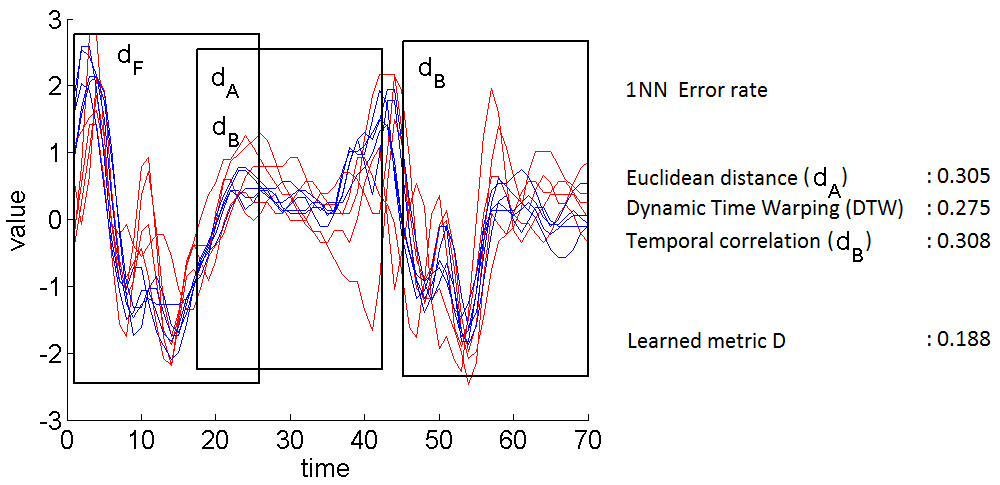
\includegraphics[width=1\linewidth]{images/SonyAIBO3}
	\caption{SonyAIBO dataset and error rate using a $k$NN ($k=1$) with standard metrics (Euclidean distance, Dynamic Time Warping, temporal correlation) and a learned combined metric $D$. The figure shows the 4 major metrics involves in the combined metric $D$ and their temporal scale (black rectangles).}
	\label{fig:SonyAIBO}
\end{figure}

% Ideally, a combined metric should answer two scenarios depending on the datasets: 1) combines several modalities at several scales; 2) select one modality at one particular scale and thus, coming back to a uni-modal and uni-scale metric framework. Figs. \ref{fig:SonyAIBO} and \ref{fig:ECG200} shows these two cases on two dataset examples used in classification of univariate time series. For SonyAIBO dataset (Fig. \ref{fig:SonyAIBO}), by learning the metric, several modalities (frequential $d_F$, behavior $d_B$ and amplitude $d_A$) at different locally temporal intervals are combined together. Thanks to this combination, the error of the 1-NN classifier is decreased: global uni-modal metrics achieves $0.305$ for $d_A$, $0.308$ for $d_B$, $0.258$ for $d_F$; and the combined metric achieves a score of 0.188. For ECG200 dataset (Fig. \ref{fig:ECG200}), the learned metric mainly includes the global behavior component $d_B$ and the error rate remains statistically the same. More detailed explanations will be given in Chapter \ref{sec:unchapitre}.

%\begin{table}[h!]
%	\small
%	\centering
%	\renewcommand{\arraystretch}{1}
%	\resizebox{0.75\textwidth}{!}{
%		\setlength{\tabcolsep}{1pt}
%		\begin{tabular}{|l|ccccc|ccc|}
%			\hline
%			& \multicolumn{5}{c|}{uni-modal metrics} & \multicolumn{2}{c}{Learned combined metrics} &  \\
%			\cline{2-9} 
%			Dataset & $d_A$ & $d_B$ & $d_F$ & $\mbox{\sc dtw}$ & $d_{B-\mbox{\sc dtw}}$ & $D$ & $D_{\mathcal{H}}$ & {\sc warp} \\
%			\hline
%			SonyAIBO            & 0.305 & 0.308 & 0.258 & 0.275 & 0.343     & \textbf{0.188} & \textbf{0.165} & $\times$   \\			
%			ECG200              & \textbf{0.120} & \textbf{0.070}& 0.160 & 0.230& 0.190    & \textbf{0.080} & \textbf{0.080} & $\times$  \\
%			\hline
%		\end{tabular}
%	}
%	\caption{1-NN  error rates for uni-modal metrics and learned combined metrics. Best equivalent performances for each dataset is indicated in bold. The considered metrics are respectively the Euclidean distance ($d_A$), the temporal correlation ($d_B$), the frequential-based distance ($d_F$), the dynamic time warping ({\sc dtw}), the temporal correlation computed on the signals re-align by the dynamic time warping ($d_{B-\mbox{\sc dtw}}$), a linear learned combined metric ($D$), a non-linear learned combined metric ($D_{\mathcal{H}}$). Last column ({\sc warp}) indicates if the learned combined metrics $D$ and $D_{\mathcal{H}}$ are computed with (\checkmark) or without warping ($\times$) }
%	\label{tab-resu2}
%\end{table}

%\begin{figure}[h!]
%\centering
%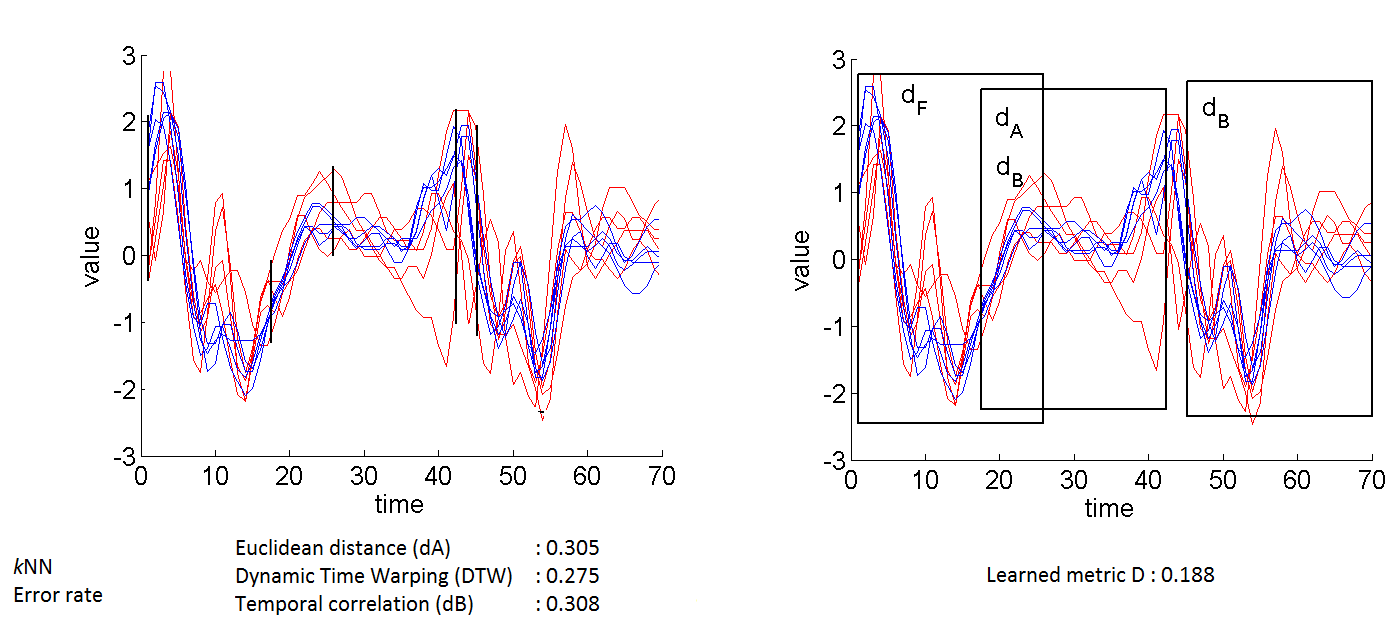
\includegraphics[width=1\linewidth]{images/SonyAIBO2}
%\caption{SonyAIBO dataset and error rate using a $k$NN with $k=1$ with standard metrics (Euclidean distance, Dynamic Time Warping, temporal correlation) (left) and a learned combined metric (right). For the learned combined metric $D$, the figure shows the 4 major metrics involves in the combination and their temporal scale (black rectangles).}
%\label{fig:SonyAIBO}
%\end{figure}
%
%
%\begin{figure}[h!]
%\centering
%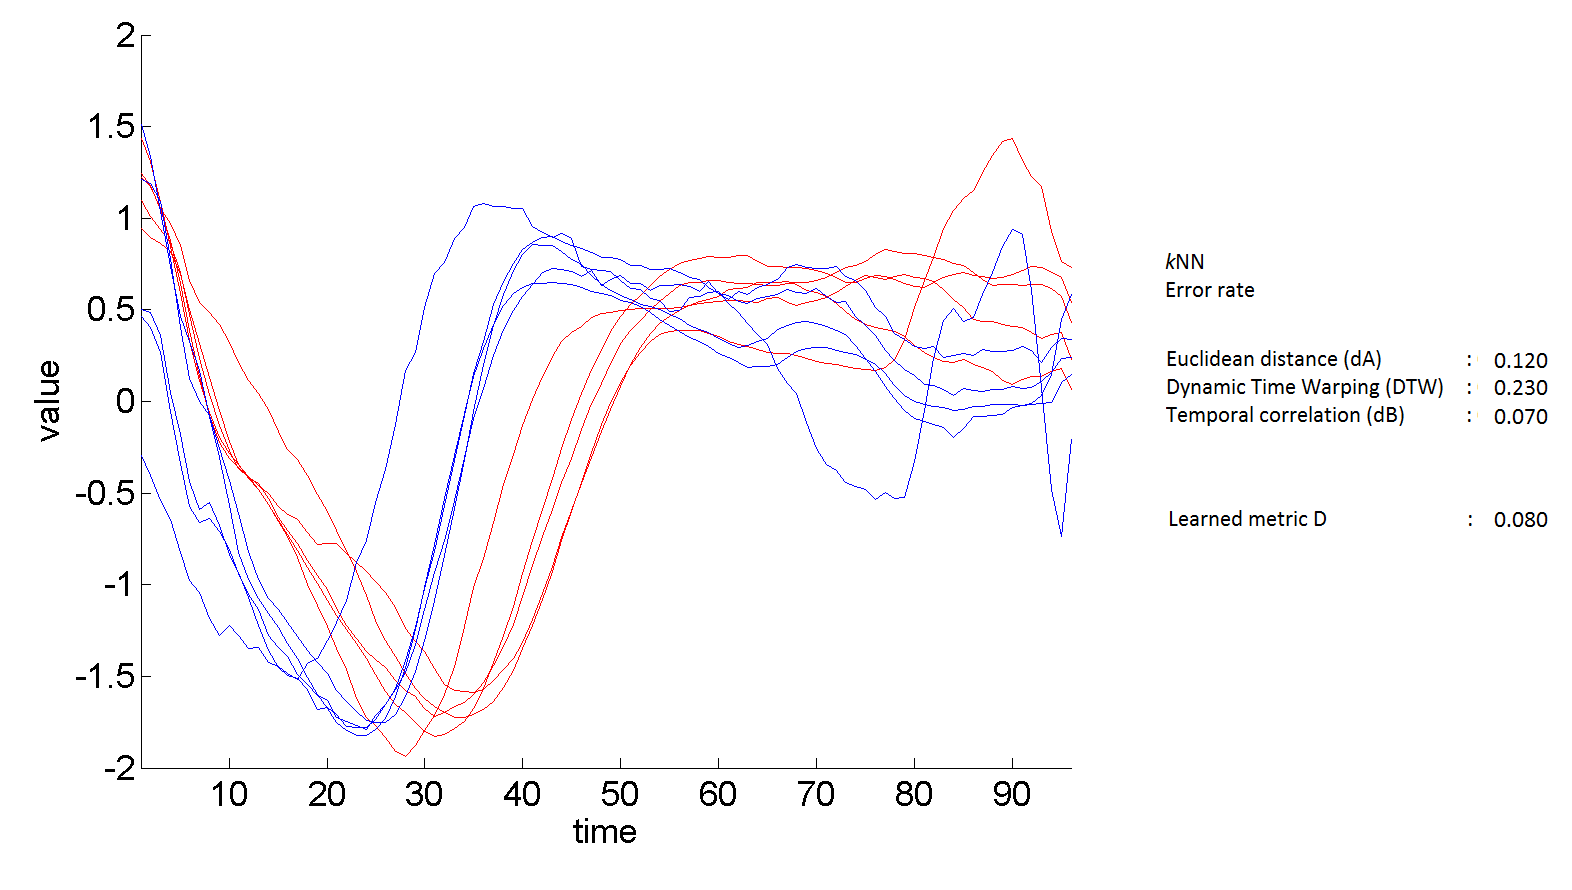
\includegraphics[width=0.7\linewidth]{images/ECG2002}
%\caption{ECG200 dataset and error rate using a $k$NN with $k=1$ with standard metrics (Euclidean distance, Dynamic Time Warping, temporal correlation) and a learned combined metric. For the learned combined metric $D$, the major discriminant feature is the behavior-based metric $d_B$ ($90\%$ of $D$) computed on a global scale (including all time series elements).}
%\label{fig:ECG200}
%\end{figure}




% \textcolor{blue}{The definition of a metric to compare samples is a fundamental issue in data analysis, pattern recognition or machine learning. For time series comparison, plenty of measures exist, most of them are designed to capture similitudes and differences based on one temporal modality, viz. by comparing time series based on their amplitudes, behaviors or frequential spectrum. For amplitude-based comparison, measures cover variants of Mahalanobis distance or the dynamic time warping to cope with delays [1, 2, 3, 4]. Other propositions refer to temporal correlations or derivative dynamic time warping for behavior-based comparison [5, 6, 7, 8, 9]. For frequential aspects, comparisons are mostly based on the Discret Fourier or Wavelet Transforms [10, 11, 12, 13]. A detailed review of the major metrics is proposed in [14]. \\
 %More recent works enhance the potential of temporal metrics by combining several modalities through a priori models as in [15, 16, 17]. For all these temporal measures, there is still room for improvement to handle complex time series by: a) integrating several modalities through a learned linear or non linear models, instead of a priori ad-hoc ones and b) involving totally or partially time series elements, rather than systematically the whole elements as operated for the most, if not all, available temporal measures.} \\


% \noindent \textbf{Motivation du Metric Learning}
%\begin{itemize}
%	\item Commencer par le metric learning en général: definition
%	\item Metric learning a eu de nombreux attraits ces dernières années, que ce soit pour les features data et les structures data (tree, graph, strings). De nombreux surveys ont été fait (Yan \& Jin, Kulis, Bellet \& al.). Elle a reçu de nombreuses recherches actives: preuves théoriques (generalization guarantees) et couvert les différents problèmes du machine learning (supervised, semi-supervised et non supervisé, online learning).
%	\item for feature data (static data) a reçu de nombreuses recherches principalement divisable en 2 catégories : linéaire et non linéaire (inspiré des SVMs, adaptation des algos ou combinaison avec des SVM). Très souvent, le problème revient à apprendre une matrice de Mahalanobis. L'approche la plus populaire qui a reçu de nombreuses extensions est celle proposée par Weinberger : LMNN.
%	\item focaliser sur le metric learning pour les données structurées : moins nombreuses et a reçu moins d'attention. Elle repose souvent sur l'optimisation de l'Edit distance
%	\item Les séries temporelles pouvant être vu comme des données structurées, les recherches dans le domaine du metric learning sont encore moins nombreuses (reprendre PRL)
%	\item terminer sur la remarque du papier de Bellet : learning richer metrics : multi-modalité
%	\item mettre les + et - de chaque méthode.
%	\item S'appuyer sur le papier de Aurélien Bellet
%\end{itemize}

Our aim is to take benefice of metric learning framework \cite{Weinberger2009a,Bellet2012} to learn a multi-modal and multi-scale temporal metric for time series nearest neighbors classification. Specifically, our objective is to learn from the data a linear or non linear function that combines several temporal modalities at several temporal scales, that satisfies metric properties (Section \ref{sec:property_metric}), and that generalizes the case of standard global metrics. \\
Metric learning can be defined as learning, from the data and for a task, a pairwise function (\textit{i.e.} a similarity, dissimilarity or a distance) to make closer samples that are expected to be similar, and far away those expected to be dissimilar. Similar and dissimilar samples, are inherently task- and application-dependent, generally given a priori and fixed during the learning process. Metric learning has become an active area of research in last decades for various machine learning problems (supervised, semi-supervised, unsupervised, online learning) and has received many interests in its theoretical background (generalization guarantees) \cite{Bellet2013a}. From the surge of recent research in metric learning, one can identify mainly two categories: the linear and non linear approaches. The former is the most popular, it defines the majority of the propositions, and focuses mainly on the Mahalanobis distance learning \cite{Weinberger2009}. The latter addresses non linear metric learning which aims to capture non linear structure in the data. In Kernel Principal Component Analysis (KPCA) \cite{Zhang2010,Chatpatanasiri2010}, the aim is to project the data into a non linear feature space and learn the metric in that projected space. In Support Vector Metric Learning (SVML) approach \cite{Xu2012}, the Mahalanobis distance is learned jointly with the learning of the SVM model in order to minimize the validation error. In general, the optimization problems are more expensive to solve, and the methods tends to favor overfitting as the constraints are generally easier to satisfy in a nonlinear kernel space. A more detailed review is done in \cite{Bellet2013a}.\\
Contrary to static data, metric learning for structured data (\textit{e.g.} sequence, time series, trees, graphs, strings) remains less numerous. While for sequence data most of the works focus on string edit distance to learn the edit cost matrix \cite{Oncina2006,Bellet2012}, metric learning for time series is still in its infancy. Without being exhaustive, major recent proposals rely on weighted variants of dynamic time warping to learn alignments under phase or amplitude constraints \cite{Reyes2011,Jeong2011,ZhangX.-L.Z.-G.Luo2014}, enlarging alignment learning framework to multiple temporal matching guided by both global and local discriminative features \cite{Frambourg2013a}. For the most of these propositions, temporal metric learning process is systematically: a) Uni-modal (amplitude-based), the divergence between aligned elements being either the Euclidean or the Mahalanobis distance and b) Uni-scale (global level) by involving the whole time series elements, which restricts its potential to capture local characteristics. We believe that perpectives for metric learning in the case of time series, should include multi-modal and multi-scale aspects.

% Bellet \& al. enlightened in \cite{Bellet2013a} perspectives for metric learning, especially, the learning of richer metrics that could take into account of the multi-modality within the data. 

% \textcolor{blue}{For this, our aim is to take benefice of Metric Learning framework [18, 19] to learn a multi-modal and multi-scale temporal metric for time series nearest neighbors classification. Specifically, we target to learn from the data a linear or non linear function that combines several temporal modalities at several temporal scales and, most importantly, that satisfies metric properties. \\
% Metric Learning framework can be defined as learning, from the data and for a task, a pairwise function (\textit{i.e.} a similarity, dissimilarity or a distance) to make closer samples that are expected to be similar, and far away those expected to be dissimilar. Similar and dissimilar samples, are inherently task- and application-dependent, generally given a priori and fixed during the learning process. From the surge of recent research in metric learning, one can identify mainly two categories: the linear and non linear approaches. The former is the most popular, it defines the majority of the propositions, and focuses mainly on the Mahalanobis distance learning. The latter addresses non linear metric learning, although more expressive, the optimization problems are more expensive to solve in general. Contrary to flat data, metric learning for structured data (\textit{e.g.} sequence, time series, trees, graphs) remains less numerous. While for sequence data most of the works focus on string edit distance to learn the edit cost matrix [20, 19], metric learning for time series is still in its infancy. Without being exhaustive, major recent proposals rely on weighted variants of dynamic time warping to learn alignments under phase or amplitude constraints [21, 22, 23], enlarging alignment learning framework to multiple temporal matching guided by both global and local discriminative features [24], or initiating a linear multi-modal metric learning solutions [25]. \\
% For the most of these propositions, temporal metric learning process is systematically: a) Uni-modal (amplitude-based), the divergence between aligned elements being either the Euclidean or the Mahalanobis distance and b) Uni-scale (global level) by involving the whole time series elements, which restricts its potential to capture local characteristics.}

% \noindent \textbf{Les problèmes que l'on attaque + Présenter dans les grandes lignes la solution}\\
% Notre travail propose une méthode qui permet de déterminer quelles sont les modalités et à quelle échelle elles interviennent. La méthode propose la combinaison de plusieurs métriques au sein d'une métrique en vue d'une classification kNN robuste. Pour cela, on propose de plonger nos individus dans un espace de dissimilarité multi-modal et multi-échelle. Sur la base de cet espace de dissimilarité, nous allons formaliser le problème d'apprentissage de la métrique combinée. \\
We propose in this work to learn a multi-modal and multi-scale temporal metric for a robust $k$-NN classifier. For this, the main idea is to embed time series into a dissimilarity space \cite{Pcekalska2002,Duin2012} where a linear function combining several modalities at different temporal scales can be learned, driven jointly by a {\sc svm} and nearest neighbors metric learning framework \cite{Weinberger2009a}. Thanks to the "kernel trick", the proposed solution is extended to non-linear temporal metric learning context. A sparse and interpretable variant of the proposed metrics confirms its ability to localize finely discriminative modalities as well as their temporal scales. In the following, the term metric is used to reference both a distance or a dissimilarity measure.

In this chapter, we first present the concept of dissimilarity space. Then, we formalize the Metric Learning problem in the Dissimilarity space ({\sc mld}) and propose three formulations: Linear Programming, Quadratic Programming, {\sc svm} approximation. Note that these formulations doesn't concern only time series and can be applied to any type of data. In the next chapter, we detail the proposed solution to learn a multi-modal and multi-scale temporal metric ({\sc m$^2$tml}) for a robust $k$-NN classifier.


%---------------------------------------------------------------------------
\section{Dissimilarity representation}
\label{sec:Pairwise_embedding}
%\begin{itemize}
%	\item Changement de l'espace
%	\item Normalisation de l'espace des paires
%	\item Label des pairwise
%\end{itemize}
Let $\{\textbf{x}_{i}, y_{i}\}_{i=1}^n$ be a set of $n$ time series labeled $y_{i}$. Let  $d_1, ..., d_h ..., d_p$ be $p$ given metrics that allow to compare samples $\textbf{x}_{i}$. For instance, in Chapter \ref{sec:Chapter_metrics}, we have proposed three types of metrics for time series: amplitude-based $d_A$, behavior-based $d_B$ and frequential-based $d_F$. Our objective is to learn a metric $D = f(d_1, \ldots , d_p)$ that combines the $p$ metrics in order to optimize the performance of a $k$-NN classifier.
 % In this section, we first introduce the dissimilarity space. Then, we give some interpretations in the dissimilarity space. 

% \subsection{Pairwise embedding}
The computation of a metric $d$, and $D$, always takes into account a pair of samples $(\textbf{x}_i,\textbf{x}_j)$. We introduce a new space representation referred as the \textbf{dissimilarity space}. In this new space, illustrated in Fig. \ref{fig:PairwiseEmbedding}, a vector $\textbf{x}_{ij}$ represents a pair of time series $(\textbf{x}_i,\textbf{x}_j)$ described by the $p$ metrics $d_h$: $\textbf{x}_{ij}=[d_1(\textbf{x}_i,\textbf{x}_j), ..., d_p(\textbf{x}_i,\textbf{x}_j)]^T$. We note $n^2$ the number of pairwise vectors $\textbf{x}_{ij}$ induced by this embedding.
%		\begin{equation*}		
%			\textbf{x}_{ij}
%			=
%			\begin{bmatrix}
%		        d_1(\textbf{x}_i,\textbf{x}_j) 	\\
%		        ... 			\\
%		       	d_p(\textbf{x}_i,\textbf{x}_j)
%		     \end{bmatrix}	    	     
%		\end{equation*}


\begin{figure}[h!]
	\begin{minipage}[b]{1.0\linewidth}
		\centering
		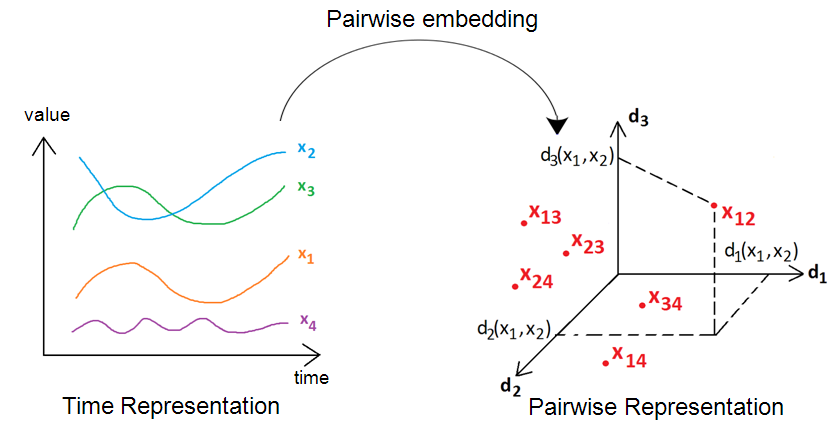
\includegraphics[width=0.9\linewidth]{images/PairwiseEmbedding}
	\end{minipage}
	\caption{Example of embedding of time series $\textbf{x}_i$ from the temporal space (left) into the dissimilarity space (right) for $p=3$ basic metrics.}
	\label{fig:PairwiseEmbedding}
\end{figure}
% In this example, a pair of time series $(\textbf{x}_1, \textbf{x}_2)$ is projected into the dissimilarity space as a vector $\textbf{x}_{12}$ described by $p=3$ basic metrics: $\textbf{x}_{12} = [d_1(\textbf{x}_1, \textbf{x}_2), d_2(\textbf{x}_1, \textbf{x}_2), d_3(\textbf{x}_1, \textbf{x}_2)]^T$.

In the dissimilarity space, a metric $D$ that combines the $p$ metrics $d_1, \ldots, d_p$ can be seen as a function of the dissimilarity space. The norm of a pairwise vector $||\textbf{x}_{ij}||$ refers to the proximity between the time series $\textbf{x}_i$ and $\textbf{x}_j$. In particular, if $||\textbf{x}_{ij}||=0$ then $\textbf{x}_j$ is identical to $\textbf{x}_i$ according to all metrics $d_h$. Note that a standard Euclidean distance between two pairwise vectors $\textbf{x}_{ij}$ and $\textbf{x}_{kl}$ in the dissimilarity space cannot give any interpretation about the proximity of the time series $\textbf{x}_i$, $\textbf{x}_j$ and $\textbf{x}_k$ and $\textbf{x}_l$ in the original space.
\mycomment[MR]{figure enlevé ici}

%---------------------------------------------------------------------------
% \subsection{Interpretation in the dissimilarity space}
%\begin{itemize}
%	\item Proximity to the origin (les individus sont identiques)
%	\item Proximity of 2 pairwise points in the dissimilarity space 
%	\item Norm in the dissimilarity space
%	\item Representation of combined metric in the dissimilarity space
%	\item perte de la classe initiale des individus. L'information qui nous reste est : les 2 individus sont de la même classe ou sont de classes différentes.
%\end{itemize}

%The interpretation of the data in the dissimilarity space is particular since the dissimilarity space is not a standard Euclidean space. The interpretation in this space requires to be careful.
%
%If $\textbf{x}_{ij}=\textbf{0}$ then $\textbf{x}_{j}$ is identical to $\textbf{x}_{i}$ according to all metrics $d_h$. The norm of the vector $\textbf{x}_{ij}$ can be interpreted as a proximity measure: the lower the norm of $\textbf{x}_{ij}$ is, the closer are the time series $\textbf{x}_{i}$ and $\textbf{x}_{j}$. Nevertheless, if two pairwise vectors $\textbf{x}_{ij}$ and $\textbf{x}_{kl}$ has their norms closed, it doesn't mean that the time series $\textbf{x}_{i}$, $\textbf{x}_{j}$, $\textbf{x}_{k}$ and $\textbf{x}_{l}$ are similar. Fig \ref{fig:ContreExample} shows an example of two pairwise vectors $\textbf{x}_{ij}$ and $\textbf{x}_{kl}$ that are close together in the dissimilarity space. However, in the temporal space, the time series $\textbf{x}_{1}$ and $\textbf{x}_{3}$ are not similar for example. It means that $\textbf{x}_i$ is as similar to $\textbf{x}_j$ as $\textbf{x}_k$ is to $\textbf{x}_l$.
%
%\begin{figure}[h!]
%\centering
%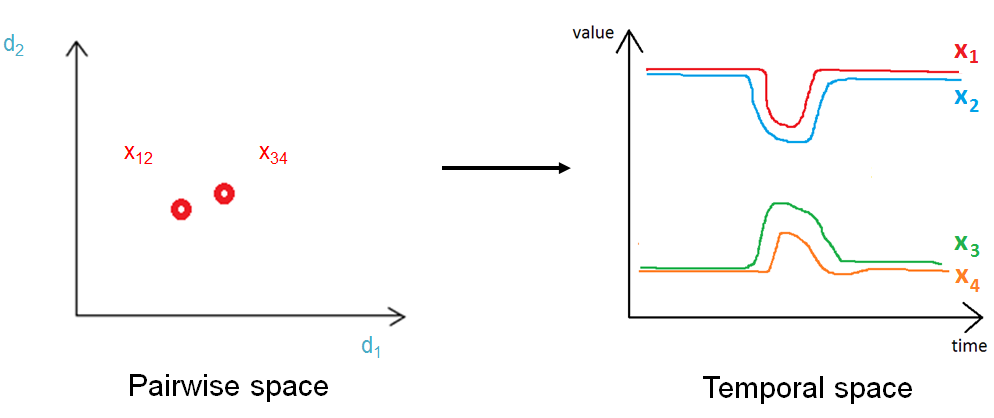
\includegraphics[width=1\linewidth]{images/ContreExample}
%\caption{Example of two pairwise vectors $\textbf{x}_{12}$ and $\textbf{x}_{34}$ close in the dissimilarity space. However, the time series $\textbf{x}_{1}$ and $\textbf{x}_{3}$ are not similar in the temporal space.}
%\label{fig:ContreExample}
%\end{figure}

%A metric $D$ that combines the $p$ metrics $d_1, \ldots, d_p$ can be seen as a function of the dissimilarity space. It can be noticed that when the time series $\textbf{x}_i$ are embedded in the pairwise, the information of their original class $y_i$ is lost. Any multi-class problem is transformed in the dissimilarity space as a binary classification problem.
%
%In the next sections, we transpose the metric learning problem for large margin nearest neighbor classifier in the dissimilarity space. We propose three formulations: Linear programming, Quadratic programming and {\sc svm}-based approach.

% Fig. \ref{fig:ContourLine} has shown the example of the representation of different combined metrics (linear ($D_{Lin}$), exponential ($D_{Exp}$) and sigmoid ($D_{Sig}$)) in the dissimilarity space for two modalities: amplitude-based ($d_A$) and behavior-based ($d_B$ and $cort$). 

\section{Metric learning framework}
In this section, we formalize our problem. We propose to define the problem of learning a metric that combines several modality at several scales in the initial space as a metric learning problem.

Our objective is to learn a metric $D$ that combines the $p$ metrics: $D=f(d_1, \ldots, d_p)$. In addition, we want the metric $D$ to optimize the performance of a $k$-NN classifier. It is based on two intuitions. First, for each sample $\textbf{x}_i$, the metric $D$ should bring closer the set its nearest neighbors $\textbf{x}_j$, called $Pull_i$. Secondly, for each sample $\textbf{x}_i$, the metric $D$ should push the set of sample $\textbf{x}_l$ that are not of the same class, called  $Push_i$. Moreover, the metric $D$ should verify the properties of a metric, \textit{i.e.}, positivity, symmetry, distinguishability, triangular inequality. Formally, the metric learning problem can be written as the following optimization problem:
\begin{equation}
\begin{aligned}
&\displaystyle 		\argmin_{D,\xi} \left\lbrace \underbrace{
	\vphantom{ \sum\limits_{\substack{i \\ j \in Pull_i \\ l \in Push_i}} \frac{1+y_{il}}{2} \xi_{ijl} }
	\sum_{\substack{i \\ j \in Pull_i}}D(\textbf{x}_{i},\textbf{x}_{j})
}_{pull}
+ C
\underbrace{
	\sum\limits_{\substack{i \\ j \in Pull_i \\ l \in Push_i}} \frac{1+y_{il}}{2} \xi_{ijl}
}
_{push} \right\rbrace  \\
&\text{s.t.  } \forall j \in Pull_i, l \in Push_i, \\
& \qquad D(\textbf{x}_{i},\textbf{x}_{l})-D(\textbf{x}_{i},\textbf{x}_{j}) \geq 1-\xi_{ijl} \\
& \qquad \xi_{ijl} \geq 0 
\label{eq:OriginalOptimizationProblem_Objective} 
\end{aligned}
\end{equation}
\noindent where $y_{il} = +1$ if $y_i \neq y_l$ and -1 otherwise, $\xi_{ijl}$ are the slack variables and $C$, the trade-off between the pull and push costs. 

This formalization is similar to the one of Large Margin Nearest Neighbors ({\sc lmnn}) proposed by Weinberger \& Saul in ~\cite{Weinberger2009}. In {\sc lmnn}, the set $Pull_i$ is defined as the $k$ nearest neighbors $\textbf{x}_j$ of the same class. The set $Push_i$ is defined by the sample $\textbf{x}_l$ that invades the perimeter defined by the set $Pull_i$, called imposters. The set $Push_i$ being sparse, \textit{i.e.}, only a subset of $\textbf{x}_{il}$ is considered in the optimization process, the computational complexity is reduced. Thus, the problem is fast to solve. However, the sets $Pull_i$ and $Push_i$ are defined and fixed during the optimization process, according to an initial metric. If the initial metric is far from the solution, the optimum might not be attained. Also, note that in {\sc lmnn}, $D(\textbf{x}_i,\textbf{x}_j)$ is replaced by $D^2(\textbf{x}_i,\textbf{x}_j)$.

We propose in our work to consider for the set $Pull_i$, a neighborhood larger than the ones of the $k$ nearest neighbors, called the $m$ neighborhood ($m \geq k$). We believe that considering a larger neighborhood during the training phase would improve the generalization properties of the learnt metric $D$ during the testing phase. Similarly, we propose to consider for the set $Push_i$, samples that are in a scope larger than the ones of the set $Pull_i$, \textit{i.e.}, considering samples $\textbf{x}_l$ that are not only imposters. For example, we could consider all samples $\textbf{x}_l$ that have a different label from $\textbf{x}_i$ ($y_l \neq y_i$). We call these samples $\textbf{x}_l$ undesired samples. However, by considering all different samples, this would increase the computational cost of the optimization problem. An intermediate solution would consider for example the neighborhood of the $m$ samples of different classes. More precisely, our solution states: $m=\alpha.k$ with $\alpha \geq 1$. Other propositions for $m$ are also possible. Fig. \ref{fig:Transposition_Pairwise2} illustrates the concept.



\begin{figure}[t]
	\centering
	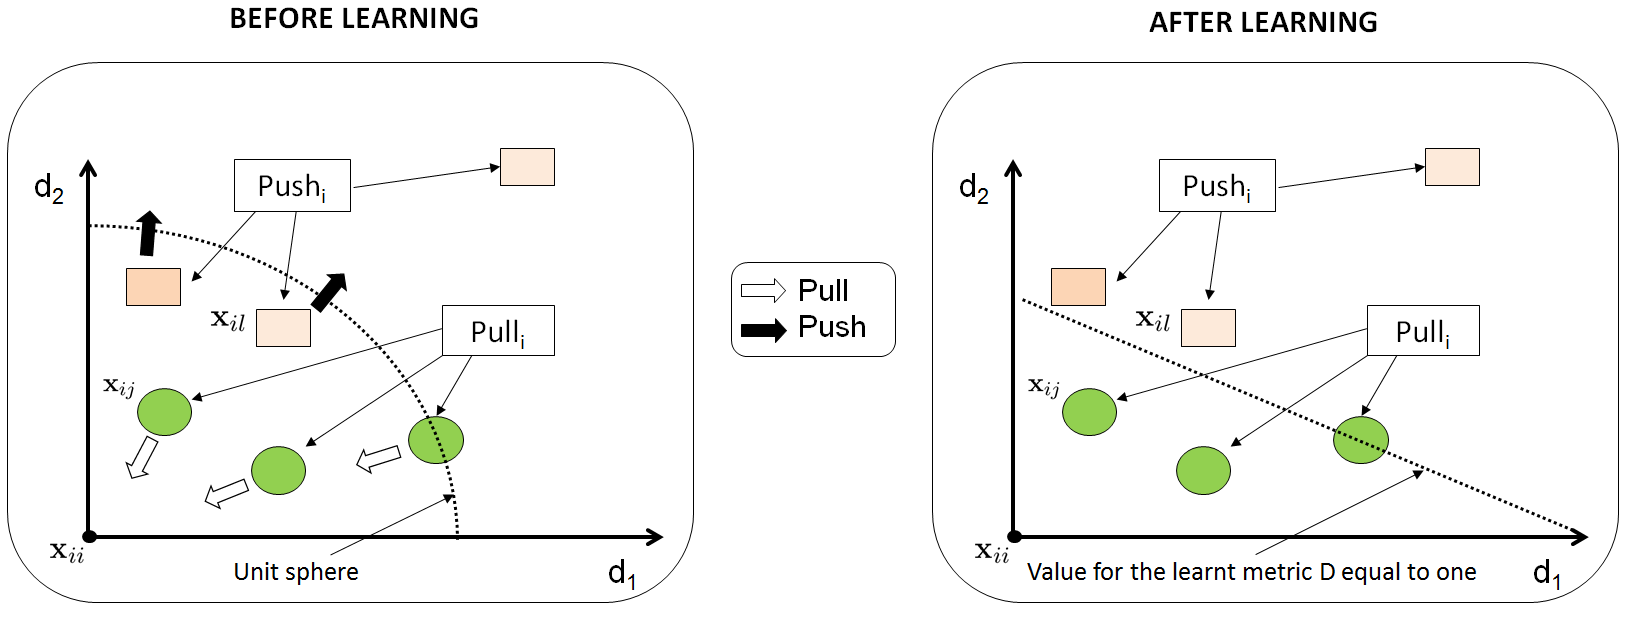
\includegraphics[width=0.9\linewidth]{images/Transposition_Pairwise3}
	\caption{Geometric representation of the metric learning problem in the dissimilarity space for a $k=3$ target neighborhood of $\textbf{x}_i$. Before learning (left), undesired samples $\textbf{x}_l$ invade the targets perimeter $\textbf{x}_j$. In the dissimilarity space, this is equivalent to have pairwise vectors $\textbf{x}_{il}$ with a norm lower to some pairwise target $\textbf{x}_{ij}$. The aim of metric learning is to push pairwise $\textbf{x}_{il}$ (black arrow) and pull pairwise $\textbf{x}_{ij}$ from the origin (white arrow).}
	\label{fig:Transposition_Pairwise2}
\end{figure}


%We first recall the standard metric learning framework proposed by Weinberger \& Saul in~\cite{Weinberger2009} referred as Large Margin Nearest Neighbors ({\sc lmnn}). The aim is to optimize the performance of the $k$-NN classifier by learning a metric $D_\textbf{M}$ parametrized by a positive semi-definite matrix $\textbf{M}$. For that, the intuition is to learn a metric $D_\textbf{M}$ that pulls for each sample $\textbf{x}_i$, its $k$ nearest neighbors, denoted $\textbf{x}_{j \rightsquigarrow i}$, while it pushes the sample $\textbf{x}_l$ of different classes ($y_l \neq y_i$), denoted $l \nrightarrow i$, that invades the perimeter of the $k$ nearest neighbors. Formally:\\
%\begin{equation}
%\begin{aligned}
%&\displaystyle 		\argmin_{\textbf{M},\xi} \text{  } \left\lbrace \underbrace{
%	\sum\limits_{i,j \rightsquigarrow i}
%	D^2_\textbf{M}(\textbf{x}_i,\textbf{x}_j)
%}_{pull}
%+
%C
%\underbrace{
%	\sum\limits_{i,j \rightsquigarrow i,l \nrightarrow i} \frac{1+y_{il}}{2} \xi_{ijl}
%}
%_{push} \right\rbrace \\
%&\text{s.t.  } \forall j \rightsquigarrow i, l \nrightarrow i, \\
%& D^2_\textbf{M}(\textbf{x}_i,\textbf{x}_l) - D^2_\textbf{M}(\textbf{x}_i,\textbf{x}_j)  \geq 1-\xi_{ijl} \\
%& \xi_{ijl} \geq 0 \\
%& \textbf{M} \succeq 0
%\label{eq:LMNN}
%\end{aligned}
%\end{equation}
%where $y_{il} = +1$ if $y_i \neq y_l$ and -1 otherwise, $\xi_{ijl}$ are the slack variables and $C$, the trade-off between the pull and push costs.
%
%Inspired from the framework of {\sc lmnn}, the intuition of our metric learning problem is to learn a metric $D$ in the dissimilarity space that pulls to the origin its $k$ nearest pairs $\textbf{x}_{ij}$ of same labels ($y_{ij}=-1$) while it pushes from the origin all pairs $\textbf{x}_{il}$ of different classes ($y_{il}=+1$). One possible way to formalize the Metric Learning problem in Dissimilarity space ({\sc mld}) is:
%
%%\begin{align}
%%	&\displaystyle 		\argmin_{D,\xi} \left\lbrace \underbrace{
%%		\vphantom{ \sum\limits_{i,j \rightsquigarrow i,l} \frac{1+y_{il}}{2} \xi_{ijl} }
%%		\sum_{i,j\rightsquigarrow i}D(\textbf{x}_{ij})
%%	}_{pull}
%%	+
%%	\underbrace{
%%		C\sum\limits_{i,j \rightsquigarrow i,l} \frac{1+y_{il}}{2} \xi_{ijl}
%%	}
%%	_{push} \right\rbrace  \label{eq:OriginalOptimizationProblem_Objective} \\
%%	&\text{s.t.  } \forall j \rightsquigarrow i, l, \nonumber \\
%%	& \qquad D(\textbf{x}_{il})-D(\textbf{x}_{ij}) \geq 1-\xi_{ijl} \label{eq:OriginalOptimizationProblem2}\\
%%	& \qquad \xi_{ijl} \geq 0 
%%	\label{eq:OriginalOptimizationProblem} 
%%\end{align}
%
%Moreover, note that several solutions in the push term are possible. First, we could consider as in {\sc lmnn} only the pairs $\textbf{x}_{il}$ that invades the neighborhood of the target pairs $\textbf{x}_{ij}$ (imposters). The advantage is that only a subset of $\textbf{x}_{il}$ is considered in the optimization process, reducing the computational complexity. Secondly, we could consider all pairs $\textbf{x}_{il}$ of different classes. In this case, it ensures that neither the imposters, nore the other pairs $\textbf{x}_{il}$ will invade the target neighborhood during the optimization process. However, taking into account all pairs $\textbf{x}_{il}$ will increase the computation complexity. Finally, note that in all cases, the targets are defined and fixed during the optimization process, according to an initial metric. Considering a larger neighborhood during the training phase could improve the generalization properties of the learnt metric $D$ during the testing phase. Fig. \ref{fig:Transposition_Pairwise2} illustrates our idea inspired from the {\sc lmnn} framework that transpose the metric learning problem in the dissimilarity space.

In the next sections, we propose three formulations: Linear problem, Non-linear problem and {\sc svm}-based approximation.



%A combination function $D$ of the metrics $d_h$ can be seen as a function in this space. In the following, we propose first to use a linear combination of $d_h$: $D(\textbf{x}_i,\textbf{x}_j) = \sum_h w_h.d_h(\textbf{x}_i,\textbf{x}_j)$. For simplification purpose, we denote $D(\textbf{x}_i,\textbf{x}_j) = D(\textbf{x}_{ij})$ and the pairwise notation gives:
%\begin{equation}
%D(\textbf{x}_i,\textbf{x}_j) = D(\textbf{x}_{ij})=\textbf{w}^T\textbf{x}_{ij}
%\label{eq:D_linear}
%\end{equation}
%where $\textbf{w}$ is the vector of weights $w_h$: $\textbf{w}=[w_1, \ldots, w_p]^T$.

\section{Problem 1}
%\begin{itemize}
%	\item Formaliser le problème sous forme d'un problème d'optimisation sous contraintes
%\end{itemize}

%We embed the $n$ time series in the dissimilarity space and define $\{\textbf{x}_{ij}, y_{ij}\}$ as the set of $N$ pairwise vectors $\textbf{x}_{ij}$ described by $p$ metrics $d_h$ and labeled $y_{ij}=+1$ if $y_{j} \neq y_{i}$ and $-1$ otherwise. Our objective is to define a metric $D$ as a linear combination of the $p$ metrics $d_h$ (Eq. \ref{eq:D_linear}). In the dissimilarity space, the metric $D$ should:
%\begin{itemize}
%	\item \textbf{pull} to the origin the $k$ nearest neighbors pairs $\textbf{x}_{ij}$ of same labels ($y_{ij} = -1$)
%	\item \textbf{push} from the origin all the pairs $\textbf{x}_{il}$ of different classes ($y_{ij} = +1$)
%\end{itemize}
%Let $\textbf{X}_{tar}$ be a $p \times (k.n)$ matrix  containing all targets $\textbf{x}_{ij}$. Fig. \ref{fig:Transposition_Pairwise} illustrates our idea to learn the metric $D$. For each time series $\textbf{x}_i$, we build the set of target pairs $\textbf{x}_{ij}$ ($j \rightsquigarrow i$) and the set of pairs $\textbf{x}_{il}$ of different class. Then, we optimize the weight vector $\textbf{w}$ so that the pairs $\textbf{x}_{ij}$ are pulled to the origin and the pairs $\textbf{x}_{il}$ are pushed from the origin.

%\begin{figure}[h!]
%	\centering
%	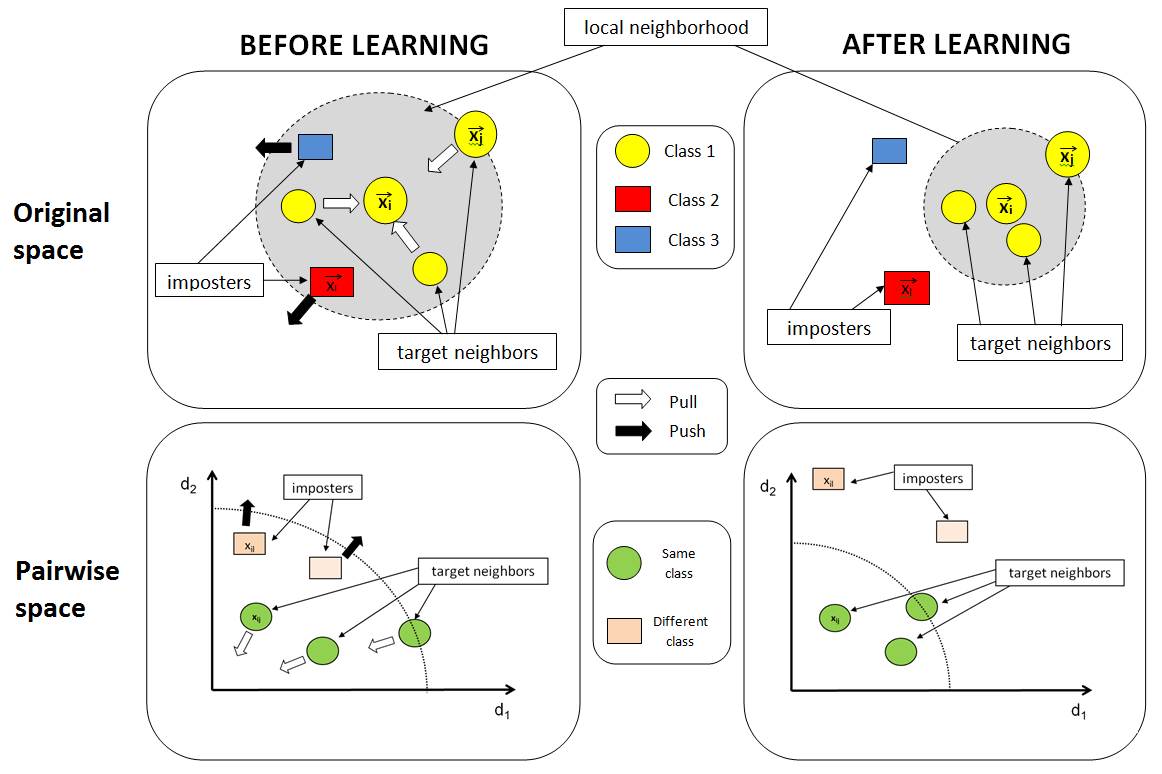
\includegraphics[width=0.9\linewidth]{images/Transposition_Pairwise}
%	\caption{Geometric representation of the adaptation of metric learning problem from the original space (top) to the dissimilarity space (bottom) for a $k=3$ target neighborhood of $\textbf{x}_i$. Before learning (left), imposters $\textbf{x}_l$ invade the targets perimeter $\textbf{x}_j$. In the dissimilarity space, this is equivalent to have pairwise vectors $\textbf{x}_{il}$ with a norm lower to some pairwise target $\textbf{x}_{ij}$. The aim of metric learning is to push pairwise $\textbf{x}_{il}$ (black arrow) and pull pairwise $\textbf{x}_{ij}$ from the origin (white arrow).}
%	\label{fig:Transposition_Pairwise}
%\end{figure}
%
%Inspired from the Large Margin Nearest Neighbors ({\sc lmnn}) framework proposed by Weinberger \& Saul in Section \ref{LMNN}, we transpose the metric learning problem into the dissimilarity space to learn a metric $D$ that combines several unimodal metric $d_h$. In our problem, the optimal metric $D$ is learned as the solution of a minimization problem, such that for each time series $\textbf{x}_i$, it pulls its targets $\textbf{x}_j$ and pushes all the samples $\textbf{x}_l$ with a different label ($y_l \neq y_i$). The Metric Learning in Dissimilarity space ({\sc mld}) problem is formalized as:
%\begin{align}
%	&\displaystyle 		\argmin_{D,\xi} \left\lbrace \underbrace{
%		\vphantom{ \sum\limits_{i,j \rightsquigarrow i,l} \frac{1+y_{il}}{2} \xi_{ijl} }
%		\sum_{i,j\rightsquigarrow i}D(\textbf{x}_{ij})
%	}_{pull}
%	+
%	\underbrace{
%		C\sum\limits_{i,j \rightsquigarrow i,l} \frac{1+y_{il}}{2} \xi_{ijl}
%	}
%	_{push} \right\rbrace  \label{eq:OriginalOptimizationProblem_Objective} \\
%	&\text{s.t.  } \forall j \rightsquigarrow i, l, \nonumber \\
%	& \qquad D(\textbf{x}_{il})-D(\textbf{x}_{ij}) \geq 1-\xi_{ijl} \label{eq:OriginalOptimizationProblem2}\\
%	& \qquad \xi_{ijl} \geq 0 
%	\label{eq:OriginalOptimizationProblem} 
%\end{align}
%
%\noindent where $\xi_{ijl}$ are the slack variables and $C$, the trade-off between the pull and push costs. The proposed {\sc mld} differs from {\sc lmnn} in which the push term in {\sc mld} considers all samples $\textbf{x}_l$ with a different label from $\textbf{x}_i$, whereas in {\sc lmnn}, only the imposters are taken into consideration (those whose invade the target perimeter). Intuitively, this due to the fact that we do not want that samples $\textbf{x}_l$ with a different class that were not at the beginning imposters, become imposters during the optimization process. By considering all the samples $\textbf{x}_l$, we ensure that at each step of the optimization process, if a sample $\textbf{x}_l$ becomes an imposter, then it will violate the constraints in Eq. \ref{eq:OriginalOptimizationProblem} and thus, its slack variables $\xi_{ijl}$ will be penalized in the objective function (Eq. \ref{eq:OriginalOptimizationProblem_Objective}) :
%\begin{itemize}
%	\item If $D(\textbf{x}_{il}) < D(\textbf{x}_{ij})$, then the pairs $\textbf{x}_{il}$ is an imposter pair that invades the neighborhood of the target pairs $\textbf{x}_{ij}$. The slack variable  $\xi_{ijl} > 1$ will be penalized in the objective function (Eq. \ref{eq:OriginalOptimizationProblem_Objective}). 
%	\item If $D(\textbf{x}_{il}) \geq D(\textbf{x}_{ij})$ but $D(\textbf{x}_{il}) \leq D(\textbf{x}_{ij})+1$, the pair $\textbf{x}_{il}$ is within the safety margin of the target pairs $\textbf{x}_{ij}$. The slack variable $ \xi_{ijl} \in [0;1]$ will have a small penalization effect in the objective function (Eq. \ref{eq:OriginalOptimizationProblem_Objective}).
%	\item If $D(\textbf{x}_{il}) > D(\textbf{x}_{ij}) +1$, $\xi_{ijl} = 0$ and the slack variable has no effect in the objective function (Eq. \ref{eq:OriginalOptimizationProblem_Objective}).
%\end{itemize}

Let $\textbf{X} = \{\textbf{x}_{ij},y_{ij}\}_{i,j=1}^n$ be a set of $n^2$ pairwise vectors $\textbf{x}_{ij}$ described by $p$ metrics: $\textbf{x}_{ij}=[d_1(\textbf{x}_i,\textbf{x}_j), ..., d_p(\textbf{x}_i,\textbf{x}_j)]^T$ labeled $y_{ij} = +1$ if $y_i \neq y_j$ and -1 otherwise. We consider a linear combination of the $p$ metrics and use the pairwise notation for simplification purpose:
\begin{equation}
D(\textbf{x}_i,\textbf{x}_j) = D(\textbf{x}_{ij})=\textbf{w}^T\textbf{x}_{ij} = \sum_h w_h.d_h(\textbf{x}_i,\textbf{x}_j)
\label{eq:D_linear}
\end{equation}
where $\textbf{w}$ is the vector of weights $w_h$: $\textbf{w}=[w_1, \ldots, w_p]^T$. We denote $\textbf{W}$ the $p \times p$ matrix which diagonal elements are $w_h$ and the other elements are zeros. We called $||\textbf{W}\textbf{x}_{ij}||_1 = \textbf{w}^T \textbf{x}_{ij}$ its $L_1$-norm. In that case, optimizing the metric $D$ is equivalent to optimizing the weight vector $\textbf{w}$. Eq. \ref{eq:OriginalOptimizationProblem_Objective} leads to the primal formulation:

\begin{equation}
\begin{aligned}
		&\displaystyle 		\argmin_{\textbf{w},\xi}
		\left\lbrace \underbrace{
		\vphantom{ \sum\limits_{i,j \rightsquigarrow i,l} \frac{1+y_{il}}{2} \xi_{ijl} }
			\sum\limits_{\substack{i \\ j \in Pull_i}} ||\textbf{W}\textbf{x}_{ij}||_1	
		}_{pull}					
		+	
		C \underbrace{				
			\sum\limits_{\substack{i \\ j \in Pull_i \\ l \in Push_i}} \frac{1+y_{il}}{2} \xi_{ijl}
		}_{push} \right\rbrace \\
 		&\text{s.t.  } \forall j \in Pull_i, l \in Push_i, \\
		& \qquad \textbf{w}^T(\textbf{x}_{il}-\textbf{x}_{ij}) \geq 1-\xi_{ijl}  \\
		& \qquad \xi_{ijl} \geq 0
		\label{eq:MMLPrimal} 
\end{aligned}
\end{equation}
%		\begin{align}
%			&\displaystyle 		\argmin_{\textbf{w},\xi}
%			\left\lbrace \underbrace{
%				\vphantom{ \sum\limits_{i,j \rightsquigarrow i,l} \frac{1+y_{il}}{2} \xi_{ijl} }
%				||\textbf{X}_{tar}^T \textbf{w}||_1	
%			}_{pull}					
%			+	
%			C \underbrace{				
%				\sum\limits_{i,j \rightsquigarrow i,l} \frac{1+y_{il}}{2} \xi_{ijl}
%			}_{push} \right\rbrace \label{eq:MMLPrimal} \\
%			&\text{s.t.  } \forall j \rightsquigarrow i,l, \nonumber \\
%			& \qquad \textbf{w}^T(\textbf{x}_{il}-\textbf{x}_{ij}) \geq 1-\xi_{ijl} \label{eq:MMLPrimal_constraint1} \\
%			& \qquad \xi_{ijl} \geq 0
%			\label{eq:MMLPrimal_constraint2}
%		\end{align}		
 %\noindent where $\textbf{X}_{tar}$ be a $p \times (m.n)$ matrix containing all targets $\textbf{x}_{ij}$, and $||\textbf{X}_{tar}^T \textbf{w}||_1=\sum_{ij} \textbf{w}^T \textbf{x}_{ij}$ denotes the $L_1$-norm of the matrix $\textbf{X}_{tar}^T \textbf{w}$. % Similarly to {\sc svm}, a $L_1$ or $L_2$ norm can be chosen in the pull term. $L_1$ norm will privilege sparse solution of $\textbf{w}$. \\

\noindent where $y_{il} = +1$ if $y_i \neq y_l$ and -1 otherwise, $\xi_{ijl}$ are the slack variables and $C$, the trade-off between the pull and push costs. We recall that the sets $Pull_i$ and $Push_i$ are defined as the $m$ nearest neighbors of the same class and of different classes. From Eq. \ref{eq:MMLPrimal} , the slack variables $\xi_{ijl}$ can  be interpreted in the dissimilarity space as follow:
% The proposed {\sc mld} differs from {\sc lmnn} in which the push term in {\sc mld} considers all samples $\textbf{x}_l$ with a different label from $\textbf{x}_i$, whereas in {\sc lmnn}, only the imposters are taken into consideration (those whose invade the target perimeter). Intuitively, this due to the fact that we do not want that samples $\textbf{x}_l$ with a different class that were not at the beginning imposters, become imposters during the optimization process. By considering all the samples $\textbf{x}_l$, we ensure that at each step of the optimization process, if a sample $\textbf{x}_l$ becomes an imposter, then it will violate the constraints in Eq. \ref{eq:OriginalOptimizationProblem} and thus, its slack variables $\xi_{ijl}$ will be penalized in the objective function (Eq. \ref{eq:OriginalOptimizationProblem_Objective}) :
\begin{itemize}
	\item If $D(\textbf{x}_{il}) = \textbf{w}^T \textbf{x}_{il} < D(\textbf{x}_{ij}) = \textbf{w}^T \textbf{x}_{ij}$, then the pairs $\textbf{x}_{il}$ is an imposter pair that invades the neighborhood of the target pairs $\textbf{x}_{ij}$. The slack variable  $\xi_{ijl} > 1$ will be penalized in the objective function. 
	\item If $D(\textbf{x}_{il}) \geq D(\textbf{x}_{ij})$ but $D(\textbf{x}_{il}) \leq D(\textbf{x}_{ij})+1$, then the pair $\textbf{x}_{il}$ is within the safety margin of the target pairs $\textbf{x}_{ij}$. The slack variable $ \xi_{ijl} \in [0;1]$ will have a small penalization effect in the objective function.
	\item If $D(\textbf{x}_{il}) > D(\textbf{x}_{ij}) +1$, $\xi_{ijl} = 0$, then the slack variables $\xi_{ijl}$ has no effect in the objective function. It corresponds to pairs $\textbf{x}_{il}$ outside of the target neighborhood.
\end{itemize}

% {\sc mld} can be seen as a large margin problem in the dissimilarity space and parallels can be done with {\sc svm}. The "pull" term acts as a regularizer which aims to minimize the norm of $\textbf{w}$. Similarly to {\sc svm}, minimizing the norm of $\textbf{w}$ is equivalent to maximizing the margin $\frac{1}{||\textbf{w}||_2}$ between target pairs $\textbf{x}_{ij}$ and pairs of different class $\textbf{x}_{il}$. 
% To ensure the positivity of the learnt metric $D$ (property 1 in Section \ref{sec:property_metric}), one possible solution is to set $w_h \geq 0$ for all $h=1...p$. This constraint can be added into the optimization problem.

\noindent Also, the norm $||\textbf{W}\textbf{x}_{ij}||_1$ can be interpreted as a linear transformation $\textbf{W}$ of the vectors $\textbf{x}_{ij}$ in the dissimilarity space. Note that we aim at ensuring the properties of a metric for the learnt metric $D$. In particular, for positivity, for all $h=1...p$, as $d_h$ are dissimilarity measures ($d_h \geq 0$), it requires that :
\begin{equation}
	w_h \geq 0
\end{equation}
This constraints is added up to the optimization problem in Eq. \ref{eq:MMLPrimal}. Finally, it can be observed that Eq. \ref{eq:MMLPrimal} is a standard constraint optimization problem involving in the objective function, the sum of a regularized (pull cost in our case) $R$ and a loss term $L$ (push cost in our case). Formally:
\begin{equation}
\begin{aligned}
	&\displaystyle 		\argmin_{\textbf{w},\xi} \left[  R(w) + L(\xi) \right] \\
	&\text{s.t. \textit{constaints} }
\end{aligned}
\end{equation}
Therefore, the problem could be extended by changing the regularizer $R$ or loss term $L$. In the following, we extend the formulation to find non-linear solution for the metric $D$. For that, we propose to change the regularizer $R$, transform the optimization problem in Eq. \ref{eq:MMLPrimal} to obtain an equivalent optimization problem that depends only on an inner product.


\section{Problem 2}
\todo[inline]{ancienne proposition. Il peut y avoir des problèmes dans l'inversibilité de la matrice}
%\begin{itemize}
%	\item Passer de la forme LP (forme primale) et par transformation, arriver à la forme duale
%	\item Montrer les similitudes avec la résolution {\sc svm}
%	\item Montrer que l'on peut kerneliser la méthode
%\end{itemize}
The primal formulation supposed that the metric $D$ is a linear combination of the metrics $d_h$. The primal formulation being similar to the one of {\sc svm}, it can be derived into its dual form to obtain non-linear solutions for $D$.
% Similarly to the SVM dual formulation (Section \ref{sec:dualSVM}), the TML primal formulation in Eq. \ref{eq:MMLPrimal} can be derived into its dual form to obtain non-linear solutions for $D$. 
For that, we consider in the objective function (Eq. \ref{eq:MMLPrimal}), the square of the $L_2$-norm on $\textbf{w}$ as the regularizer term, $\frac{1}{2}||\textbf{X}_{tar}^T \textbf{w}||_2^2$:

\begin{align}
	&\displaystyle 		\argmin_{\textbf{w},\xi}
	\left\lbrace \frac{1}{2}||\textbf{X}_{tar}^T \textbf{w}||_2^2						
	+					
	C\sum\limits_{i,j \rightsquigarrow i,l} \frac{1+y_{il}}{2}.\xi_{ijl}
	\right\rbrace  \label{eq:MMLPrimalL2} \\
	&\text{s.t.  } \forall j \rightsquigarrow i, y_l\neq y_i, \nonumber \\
	& \qquad \textbf{w}^T(\textbf{x}_{il}-\textbf{x}_{ij}) \geq 1-\xi_{ijl} \label{eq:MMLPrimalL2_constraints1} \\
	& \qquad \xi_{ijl} \geq 0 \label{eq:MMLPrimalL2_constraints2}
\end{align}
This formulation can be reduced to the minimization of the following Lagrange function $L(\textbf{w},\xi,\boldsymbol{\alpha},\textbf{r})$, consisting of the sum of the objective function (Eq. \ref{eq:MMLPrimalL2}) and the constraints (Eqs. \ref{eq:MMLPrimalL2_constraints1} and \ref{eq:MMLPrimalL2_constraints2}) multiplied by their respective Lagrange multipliers $\boldsymbol{\alpha}$ and $\textbf{r}$:
\begin{equation}
\begin{aligned}
L(\textbf{w},\xi,\boldsymbol{\alpha},\textbf{r}) 
= & 
\frac{1}{2}||\textbf{X}_{tar}^T \textbf{w}||_2^2
+ C \sum\limits_{ijl} \frac{1+y_{il}}{2} \xi_{ijl} - \sum\limits_{ijl}r_{ijl} \xi_{ijl} \\
&  - \sum\limits_{ijl} \alpha_{ijl}\left( \textbf{w}^T(\textbf{x}_{il}-\textbf{x}_{ij}-1+\xi_{ijl} \right))
\label{eq:OptimizationDual}
\end{aligned}
\end{equation}
\noindent where $\alpha_{ijl} \geq 0$ and $r_{ijl} \geq 0$ are the Lagrange multipliers. At the minimum value of $L(\textbf{w},\xi,\boldsymbol{\alpha},\textbf{r})$, we assume the derivatives with respect to $\textbf{w}$ and $\xi_{ijl}$ are set to zero:
\begin{align*}
	\frac{\partial L}{\partial \textbf{w}} 
	& = 
	\textbf{X}_{tar}^T \textbf{X}_{tar} \textbf{w} 
	- \sum\limits_{ijl} \alpha_{ijl}(\textbf{x}_{il}-\textbf{x}_{ij}) 
	= 0 \\
	\frac{\partial L}{\partial \xi_{ijl}} & = C - \alpha_{ijl} - r_{ijl} = 0
\end{align*}
\noindent that leads to:
\begin{align}
	& \textbf{w} = (\textbf{X}_{tar} \textbf{X}_{tar}^T)^{-1}  
	\sum\limits_{ijl} \alpha_{ijl}(\textbf{x}_{il}-\textbf{x}_{ij}) \label{Eq:eqn_w} 
	\\ 
	& r_{ijl} = C - \alpha_{ijl} \label{Eq:eqn_w2}
\end{align}

\noindent Substituting Eq. \ref{Eq:eqn_w} and \ref{Eq:eqn_w2} back into $L(\textbf{w},\xi,\boldsymbol{\alpha},\textbf{r})$ in Eq. \ref{eq:OptimizationDual}, we get the dual formulation\footnote{complete details of the calculations in Appendix \ref{chap:app:qp_resolution}}:
\begin{align}
	&\displaystyle \argmax_{\boldsymbol{\alpha}} \left\lbrace 
	\sum\limits_{ijl} \alpha_{ijl} 
	- \frac{1}{2} \sum\limits_{ijl} \sum\limits_{i'j'l'}
	\alpha_{ijl} \alpha_{i'j'l'}
	(\textbf{x}_{il}-\textbf{x}_{ij})^T
	(\textbf{X}_{tar} \textbf{X}_{tar}^T)^{-1}
	(\textbf{x}_{i'l'}-\textbf{x}_{i'j'}) \right\rbrace \label{eq:OptimDual} \\
	&\text{s.t. $\forall$ $i$, $j \rightsquigarrow i$ and $l$ s.t. $y_{il}=+1$:} \nonumber \\
	& 0 \leq \alpha_{ijl} \leq C
	\label{eq:OptimDualconstraint}
\end{align}

\noindent For any new pair of samples $\textbf{x}_{i'}$ and $\textbf{x}_{j'}$, the resulting metric $D$ writes: 
\begin{align}
	D(\textbf{x}_{i'j'}) = & \textbf{w}^T \textbf{x}_{i'j'} \label{eq:D1} \\
	D(\textbf{x}_{i'j'}) = & \sum\limits_{ijl} \alpha_{ijl} 
	(\textbf{x}_{il}-\textbf{x}_{ij})^T
	(\textbf{X}_{tar}\textbf{X}_{tar}^T)^{-1}
	\textbf{x}_{i'j'}
	\label{eq:D1_2}
\end{align}
% At the optimality, only the triplet $(\textbf{x}_{il}-\textbf{x}_{ij})$ which $\textbf{x}_{il}$ that has the $L_2$ norm greater than 1 and that lies closest to the unit circle of targets $\textbf{x}_{ij}$ or those triplets that have a $L_2$ norm lower that one, have $\alpha_{ijl} > 0$. These points are the support vectors. 
with $\textbf{w}$ defined in Eq. \ref{Eq:eqn_w}. At the optimality, only the triplets $(\textbf{x}_{il}-\textbf{x}_{ij})$ with $\alpha_{ijl} > 0$ are considered as the support vectors. The direction $\textbf{w}$ of the metric $D$ is lead by these triplets. All other triplets have $\alpha_{ijl} = 0$ (non-support vector), and the metric $D$ is independent from this triplets. If we remove some of the non-support vectors, the metric $D$ remains unaffected. From the viewpoint of optimization theory, we can also see this from the Karush-Kuhn-Tucker (KKT) conditions: the complete set of conditions which must be satisfied at the optimum of a constrained optimization problem. At the optimum, the Karush-Kuhn-Tucker (KKT) conditions apply, in particular:
\begin{equation*}
	\alpha_{ijl} (\textbf{w}^T (\textbf{x}_{il}-\textbf{x}_{ij}) - 1 + \xi_{ijl}) = 0
\end{equation*}

\noindent from which we deduce that either $\textbf{w}^T(\textbf{x}_{il}-\textbf{x}_{ij}) > 1 $ and $\alpha_{ijl} = 0$ (the triplet $(\textbf{x}_{il}-\textbf{x}_{ij})$ is a non-support vector), or $\textbf{w}^T(\textbf{x}_{il}-\textbf{x}_{ij}) = 1- \xi_{ijl}$ and $\alpha_{ijl} > 0$ (the triplet is a support vector). Therefore, the learned metric $D$ is a combination of scalar products between new pairs $\textbf{x}_{i'j'}$ and a few number of triplets $\textbf{x}_{ijl}$ of the training set. \\


\noindent \textbf{Extension to non-linear function of $D$} \\
\noindent The above formula can extended to non-linear function for the metric $D$. The dual formulation in Eq.~\ref{eq:OptimDual} only relies on the inner product $(\textbf{x}_{i'l'}-\textbf{x}_{i'j'})^T (\textbf{X}_{tar} \textbf{X}_{tar}^T)^{-1} (\textbf{x}_{il}-\textbf{x}_{ij})$. We can hence apply the kernel trick on Eqs. \ref{eq:D1} and \ref{eq:D1_2} to find non-linear solutions for $D$:
\begin{align}
	D(\textbf{x}_{i'j'}) & = \textbf{w}^T \phi(\textbf{x}_{i'j'}) \nonumber\\
	D(\textbf{x}_{i'j'}) &= \sum\limits_{ijl} \alpha_{ijl} 
	\phi(
	\textbf{x}_{il}-\textbf{x}_{ij}
	)
	\phi(	
	\textbf{x}_{i'j'}
	) \nonumber \\
	D(\textbf{x}_{i'j'}) &= \sum\limits_{ijl} \alpha_{ijl} 
	K(\textbf{x}_{il}-\textbf{x}_{ij} ; \textbf{x}_{i'j'}) \nonumber				
\end{align}
These equations suppose that the null vector $\textbf{0}$ in the original space is transformed through the transformation $\phi$ into the null vector: $\phi(\textbf{0})=\textbf{0}$ in the feature space. We recall that $D(\textbf{x}_{ii} = \textbf{0})$ is expected to be equal to zero (distinguishability property in Section \ref{sec:property_metric}). However, if the vectors $\textbf{x}_{ij}$ are projected in a feature space by a transformation $\phi$, it doesn't guarantee that $\phi(\textbf{0})=\textbf{0}$. Fig. \ref{fig:Kernel_nonHomogene} illustrates the idea for a polynomial kernel in which $\phi(\textbf{0}) = [0, 0, 0, 1]^T$. Thus, the metric measure needs to be computed in the feature space relatively to the projection of $\phi(\textbf{0})$. This is done by adding a term $\textbf{w}^T \phi(\textbf{0})$ to Eqs. \ref{eq:D1} and \ref{eq:D1_2}:

\begin{align}
	D(\textbf{x}_{i'j'}) & = \textbf{w}^T \phi(\textbf{x}_{i'j'}) - \textbf{w}^T \phi(\textbf{0})\\
	D(\textbf{x}_{i'j'}) &= \sum\limits_{ijl} \alpha_{ijl} 
	\phi(
	\textbf{x}_{il}-\textbf{x}_{ij}
	)
	\phi(	
	\textbf{x}_{i'j'}-\textbf{x}_{ij}
	) 
	-
	\sum\limits_{ijl} \alpha_{ijl} 
	\phi(
	\textbf{x}_{il}-\textbf{x}_{ij}
	)
	\phi(	
	\textbf{0}-\textbf{x}_{ij}
	) 				
	\\
	D(\textbf{x}_{i'j'}) &= \sum\limits_{ijl} \alpha_{ijl} 
	K
	\left( 
	\textbf{x}_{il}-\textbf{x}_{ij}
	;	
	\textbf{x}_{i'j'}-\textbf{x}_{ij}
	\right) 		
	-
	\sum\limits_{ijl} \alpha_{ijl} 
	K
	\left( 
	\textbf{x}_{il}-\textbf{x}_{ij}
	;	
	\textbf{0}-\textbf{x}_{ij}
	\right) 		
	\label{Eq:nonlinearD}		
\end{align}
%For any new pair of samples $\textbf{x}_{i'}$ and $\textbf{x}_{j'}$, the resulting metric $D$ writes: 
%\begin{align}
%D(\textbf{x}_{i'j'}) = & \textbf{w}^T \textbf{x}_{i'j'} - \textbf{w}^T \textbf{0} 
%\nonumber \\
%D(\textbf{x}_{i'j'}) = & \sum\limits_{ijl} \alpha_{ijl} 
%(\textbf{x}_{il}-\textbf{x}_{ij})^T
%(\textbf{X}_{tar}\textbf{X}_{tar}^T)^{-1}
%\textbf{x}_{i'j'} 
%-
%\sum\limits_{ijl} \alpha_{ijl} 
%(\textbf{x}_{il}-\textbf{x}_{ij})^T
%(\textbf{X}_{tar}\textbf{X}_{tar}^T)^{-1}
%\textbf{0}
%\nonumber \\
%& -\sum\limits_{ijl} \alpha_{ijl} 
%(\textbf{x}_{il}-\textbf{x}_{ij})^T
%(\textbf{X}_{tar}\textbf{X}_{tar}^T)^{-1}\textbf{x}_{ij} + \sum\limits_{ijl} \alpha_{ijl} 
%(\textbf{x}_{il}-\textbf{x}_{ij})^T
%(\textbf{X}_{tar}\textbf{X}_{tar}^T)^{-1}\textbf{x}_{ij}
%\nonumber \\
%D(\textbf{x}_{i'j'}) = & \sum\limits_{ijl} \alpha_{ijl} 
%(\textbf{x}_{il}-\textbf{x}_{ij})^T
%(\textbf{X}_{tar}\textbf{X}_{tar}^T)^{-1}
%(\textbf{x}_{i'j'}-\textbf{x}_{ij}) 
%\nonumber \\
%& - \sum\limits_{ijl} \alpha_{ijl} 
%(\textbf{x}_{il}-\textbf{x}_{ij})^T
%(\textbf{X}_{tar}\textbf{X}_{tar}^T)^{-1}
%(\textbf{0}-\textbf{x}_{ij}) \label{eq:D2}
%\end{align}
\noindent where $\textbf{0}$ denotes the null vector. The resulting metric $D$ is made of two terms. The first one, $\textbf{w}^T \phi(\textbf{x}_{i'j'})$, is the metric measure for a new pair $\textbf{x}_{i'j'}$. The second term, $\textbf{w}^T \phi(\textbf{0})$, adapts the metric measure relatively to the origin point. 

\begin{figure}[h!]
	\centering
	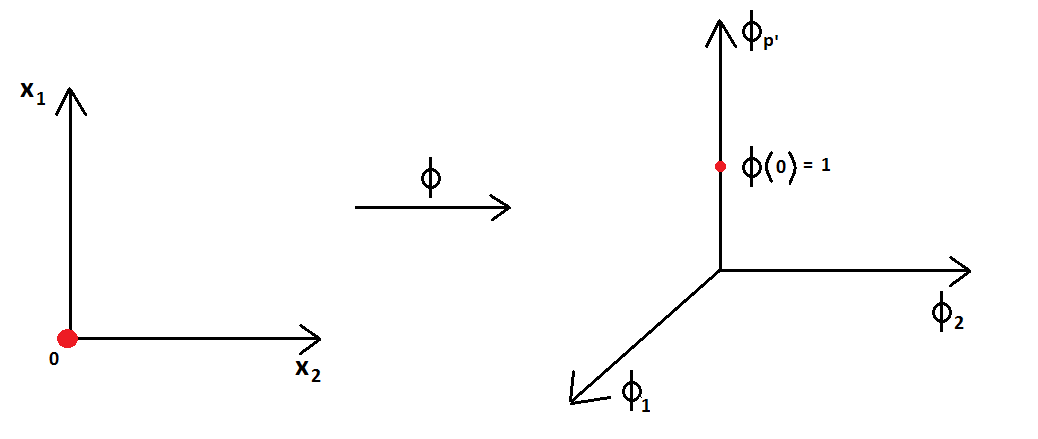
\includegraphics[width=0.9\linewidth]{images/Kernel_nonHomogene}
	\caption{Illustration of samples in $\mathbb{R}^2$. The transformation $\phi$ for a polynomial kernel $K(\textbf{x}_i,\textbf{x}_j)=(\textbf{x}_i^T \textbf{x}_j + c)^d$ with $c=1$ and $d=2$ can be written explicitly: $\phi(\textbf{x}_i)= [x_{i1}^2, x_{i2}^2, \sqrt{2} x_{i1} x_{i2}, 1]^T$. The origin point $\textbf{x}_i=[0,0]^T$ is projected in the Hilbert space as $\phi(\textbf{x}_i=\textbf{0}) = [0, 0, 0, 1]^T$.}
	\label{fig:Kernel_nonHomogene}
\end{figure}

However, to define proper metrics that respects the properties of metrics (Section \ref{sec:property_metric}), specific kernels must be used. Our work don't propose any solutions to this problem but open the field for new research on this topic. 


\section{Problem 3}
%\begin{itemize}
%	\item Passer de la forme LP (forme primale) et par transformation, arriver à la forme duale
%	\item Montrer les similitudes avec la résolution {\sc svm}
%	\item Montrer que l'on peut kerneliser la méthode
%\end{itemize}

\todo[inline]{Nouvelle proposition qui change la régularisation et permet de ne plus obtenir de problème d'inversibilité de la matrice}

The formulation in Eq. \ref{eq:MMLPrimal} suppose that the metric $D$ is a linear combination of the metrics $d_h$. The primal formulation being similar to the one of {\sc svm}, it can be derived into its dual form to obtain non-linear solutions for $D$.

\noindent Let $\textbf{X}_{tar}$ be a $(m.n) \times p$ matrix containing the pairwise vector $\textbf{x}_{ij} \in Pull_i$. Let $\textbf{M} = Diag(\textbf{X}_{tar}^T\textbf{X}_{tar}):$
\begin{equation}
	\textbf{M} = Diag(\textbf{X}_{tar}^T\textbf{X}_{tar}) = 
	\begin{bmatrix} 
		\sum\limits_{\substack{i \\ j \in Pull_i}} d_1^2(\textbf{x}_{ij}) 		&  	& 0 \\ 
			& \ddots 	&  \\ 
		0 		&  	& \sum\limits_{\substack{i \\ j \in Pull_i}} d_p^2(\textbf{x}_{ij})
		\end{bmatrix}
\end{equation}
% Similarly to the SVM dual formulation (Section \ref{sec:dualSVM}), the TML primal formulation in Eq. \ref{eq:MMLPrimal} can be derived into its dual form to obtain non-linear solutions for $D$. 

\noindent Then, we change the regularizer in the objective function of Eq. \ref{eq:MMLPrimal}:
\begin{equation}
	R(w) = \frac{1}{2} \textbf{w}^T \textbf{M} \textbf{w} = \frac{1}{2} \sum\limits_{h=1}^{p} \sum\limits_{\substack{i \\ j \in Pull_i}} w_h^2 d_h^2(\textbf{x}_{ij})
\end{equation}
\noindent From this, the optimization problem becomes:
\begin{align}
	&\displaystyle 		\argmin_{\textbf{w},\xi}
	\left\lbrace \frac{1}{2} \textbf{w}^T \textbf{M} \textbf{w}					
	+					
	C\sum\limits_{i,j \rightsquigarrow i,l} \frac{1+y_{il}}{2} \xi_{ijl}
	\right\rbrace  \label{eq:MMLPrimalL2} \\
	&\text{s.t.  } \forall j \rightsquigarrow i, l, \nonumber \\
	& \qquad \textbf{w}^T(\textbf{x}_{il}-\textbf{x}_{ij}) \geq 1-\xi_{ijl} \label{eq:MMLPrimalL2_constraints1} \\
	& \qquad \xi_{ijl} \geq 0 \label{eq:MMLPrimalL2_constraints2}
\end{align}
This formulation can be reduced to the minimization of the following Lagrange function $L(\textbf{w},\xi,\boldsymbol{\alpha},\textbf{r})$, consisting of the sum of the objective function (Eq. \ref{eq:MMLPrimalL2}) and the constraints (Eqs. \ref{eq:MMLPrimalL2_constraints1} and \ref{eq:MMLPrimalL2_constraints2}) multiplied by their respective Lagrange multipliers $\boldsymbol{\alpha}$ and $\textbf{r}$:
\begin{equation}
\begin{aligned}
	L(\textbf{w},\xi,\boldsymbol{\alpha},\textbf{r}) 
	= & 
	\frac{1}{2} \textbf{w}^T \textbf{M} \textbf{w}
	+ C \sum\limits_{ijl} \frac{1+y_{il}}{2} \xi_{ijl} - \sum\limits_{ijl}r_{ijl} \xi_{ijl} \\
	&  - \sum\limits_{ijl} \alpha_{ijl}\left( \textbf{w}^T(\textbf{x}_{il}-\textbf{x}_{ij}-1+\xi_{ijl} \right))
	\label{eq:OptimizationDual}
\end{aligned}
\end{equation}
\noindent where $\alpha_{ijl} \geq 0$ and $r_{ijl} \geq 0$ are the Lagrange multipliers. At the minimum value of $L(\textbf{w},\xi,\boldsymbol{\alpha},\textbf{r})$, we assume the derivatives with respect to $\textbf{w}$ and $\xi_{ijl}$ are set to zero:

\begin{align*}
\frac{\partial L}{\partial \textbf{w}} 
& = 
\textbf{M} \textbf{w} 
- \sum\limits_{ijl} \alpha_{ijl}(\textbf{x}_{il}-\textbf{x}_{ij}) 
= 0 \\
\frac{\partial L}{\partial \xi_{ijl}} & = C - \alpha_{ijl} - r_{ijl} = 0
\end{align*}
\noindent The matrix $\textbf{M}$ being diagonale, it is thus inversible. The equations leads to:
\begin{align}
& \textbf{w} = \textbf{M}^{-1}  
\sum\limits_{ijl} \alpha_{ijl}(\textbf{x}_{il}-\textbf{x}_{ij}) \label{Eq:eqn_w} 
\\ 
& r_{ijl} = C - \alpha_{ijl} \label{Eq:eqn_w2}
\end{align}

\noindent Substituting Eq. \ref{Eq:eqn_w} and \ref{Eq:eqn_w2} back into $L(\textbf{w},\xi,\boldsymbol{\alpha},\textbf{r})$ in Eq. \ref{eq:OptimizationDual}, we get the {\sc mld} dual formulation\footnote{complete details of the calculations in Appendix \ref{chap:app:qp_resolution}}:

\begin{align}
&\displaystyle \argmax_{\boldsymbol{\alpha}} \left\lbrace 
\sum\limits_{ijl} \alpha_{ijl} 
- \frac{1}{2} \sum\limits_{ijl} \sum\limits_{i'j'l'}
\alpha_{ijl} \alpha_{i'j'l'}
(\textbf{x}_{il}-\textbf{x}_{ij})^T
\textbf{M}^{-1}
(\textbf{x}_{i'l'}-\textbf{x}_{i'j'}) \right\rbrace \label{eq:OptimDual} \\
&\text{s.t. $\forall$ $i$, $j \rightsquigarrow i$ and $l$ s.t. $y_{il}=+1$:} \nonumber \\
& 0 \leq \alpha_{ijl} \leq C
\label{eq:OptimDualconstraint}
\end{align}

\noindent For any new pair of samples $\textbf{x}_{i'}$ and $\textbf{x}_{j'}$, the resulting metric $D$ writes: 
\begin{align}
D(\textbf{x}_{i'j'}) = & \textbf{w}^T \textbf{x}_{i'j'} \label{eq:D1} \\
D(\textbf{x}_{i'j'}) = & \sum\limits_{ijl} \alpha_{ijl} 
(\textbf{x}_{il}-\textbf{x}_{ij})^T
\textbf{M}^{-1}
\textbf{x}_{i'j'}
\label{eq:D1_2}
\end{align}
% At the optimality, only the triplet $(\textbf{x}_{il}-\textbf{x}_{ij})$ which $\textbf{x}_{il}$ that has the $L_2$ norm greater than 1 and that lies closest to the unit circle of targets $\textbf{x}_{ij}$ or those triplets that have a $L_2$ norm lower that one, have $\alpha_{ijl} > 0$. These points are the support vectors. 
with $\textbf{w}$ defined in Eq. \ref{Eq:eqn_w}. At the optimality, only the triplets $(\textbf{x}_{il}-\textbf{x}_{ij})$ with $\alpha_{ijl} > 0$ are considered as the support vectors. The direction $\textbf{w}$ of the metric $D$ is lead by these triplets. All other triplets have $\alpha_{ijl} = 0$ (non-support v ector), and the metric $D$ is independent from this triplets. If we remove some of the non-support vectors, the metric $D$ remains unaffected. From the viewpoint of optimization theory, we can also see this from the Karush-Kuhn-Tucker (KKT) conditions: the complete set of conditions which must be satisfied at the optimum of a constrained optimization problem. At the optimum, the Karush-Kuhn-Tucker (KKT) conditions apply, in particular:
\begin{equation*}
\alpha_{ijl} (\textbf{w}^T (\textbf{x}_{il}-\textbf{x}_{ij}) - 1 + \xi_{ijl}) = 0
\end{equation*}

\noindent from which we deduce that either $\textbf{w}^T(\textbf{x}_{il}-\textbf{x}_{ij}) > 1 $ and $\alpha_{ijl} = 0$ (the triplet $(\textbf{x}_{il}-\textbf{x}_{ij})$ is a non-support vector), or $\textbf{w}^T(\textbf{x}_{il}-\textbf{x}_{ij}) = 1- \xi_{ijl}$ and $\alpha_{ijl} > 0$ (the triplet is a support vector). Therefore, the learned metric $D$ is a combination of scalar products between new pairs $\textbf{x}_{i'j'}$ and a few number of triplets $\textbf{x}_{ijl}$ of the training set. \\


\noindent \textbf{Extension to non-linear function of $D$} \\
\noindent The above formula can extended to non-linear function for the metric $D$. The dual formulation in Eq.~\ref{eq:OptimDual} only relies on the inner product $(\textbf{x}_{i'l'}-\textbf{x}_{i'j'})^T \textbf{M}^{-1} (\textbf{x}_{il}-\textbf{x}_{ij})$. We can hence apply the kernel trick on Eqs. \ref{eq:D1} and \ref{eq:D1_2} to find non-linear solutions for $D$. As $\textbf{M}^{-1}$ is a diagonal matrix, it is inversible and can be written $\textbf{M}^{-1} = \textbf{M}^{-\frac{1}{2}} \textbf{M}^{-\frac{1}{2}}$. Thus:
\begin{align}
		(\textbf{x}_{i'l'}-\textbf{x}_{i'j'})^T \textbf{M}^{-1} (\textbf{x}_{il}-\textbf{x}_{ij}) 
		& = (\textbf{x}_{i'l'}-\textbf{x}_{i'j'})^T \textbf{M}^{-\frac{1}{2}} \textbf{M}^{-\frac{1}{2}} (\textbf{x}_{il}-\textbf{x}_{ij})	\nonumber	\\
		& = \left( \textbf{M}^{-\frac{1}{2}} (\textbf{x}_{i'l'}-\textbf{x}_{i'j'}) \right)^T \left( \textbf{M}^{-\frac{1}{2}} (\textbf{x}_{il}-\textbf{x}_{ij}) \right) \nonumber \\
		& = <\textbf{M}^{-\frac{1}{2}} (\textbf{x}_{i'l'}-\textbf{x}_{i'j'}) ; \textbf{M}^{-\frac{1}{2}} (\textbf{x}_{il}-\textbf{x}_{ij}) > \nonumber \\
		& = K(\textbf{M}^{-\frac{1}{2}} (\textbf{x}_{i'l'}-\textbf{x}_{i'j'}) ;  \textbf{M}^{-\frac{1}{2}} (\textbf{x}_{il}-\textbf{x}_{ij}) ) \nonumber
\end{align}
\noindent By replacing the inner product by a kernel back into Eqs. \ref{eq:D1} \& \ref{eq:D1_2}, we obtain:
\begin{align}
D(\textbf{x}_{i'j'}) & = \textbf{w}^T \phi(\textbf{M}^{-\frac{1}{2}}\textbf{x}_{i'j'}) \nonumber\\
D(\textbf{x}_{i'j'}) &= \sum\limits_{ijl} \alpha_{ijl} 
\phi( \textbf{M}^{-\frac{1}{2}}
(\textbf{x}_{il}-\textbf{x}_{ij})
)
\phi(	
\textbf{M}^{-\frac{1}{2}} \textbf{x}_{i'j'}
) \nonumber \\
D(\textbf{x}_{i'j'}) &= \sum\limits_{ijl} \alpha_{ijl} 
K(\textbf{M}^{-\frac{1}{2}} (\textbf{x}_{il}-\textbf{x}_{ij}) ; \textbf{M}^{-\frac{1}{2}}\textbf{x}_{i'j'}) \nonumber				
\end{align}
These equations suppose that the null vector $\textbf{0}$ in the original space is transformed through the transformation $\phi$ into the null vector: $\phi(\textbf{0})=\textbf{0}$ in the feature space. We recall that $D(\textbf{x}_{ii} = \textbf{0})$ is expected to be equal to zero (distinguishability property in Section \ref{sec:property_metric}). However, if the vectors $\textbf{x}_{ij}$ are projected in a feature space by a transformation $\phi$, it doesn't guarantee that $\phi(\textbf{0})=\textbf{0}$. Fig. \ref{fig:Kernel_nonHomogene} illustrates the idea for a polynomial kernel in which $\phi(\textbf{0}) = [0, 0, 0, 1]^T$. Thus, the metric measure needs to be computed in the feature space relatively to the projection of $\phi(\textbf{0})$. This is done by adding a term $\textbf{w}^T \phi(\textbf{0})$ to Eqs. \ref{eq:D1} and \ref{eq:D1_2}:
\begin{align}
D(\textbf{x}_{i'j'}) & = \textbf{w}^T \phi(\textbf{M}^{-\frac{1}{2}}\textbf{x}_{i'j'}) - \textbf{w}^T \phi(\textbf{0})\\
D(\textbf{x}_{i'j'}) &= \sum\limits_{ijl} \alpha_{ijl} 
\phi(\textbf{M}^{-\frac{1}{2}}(
\textbf{x}_{il}-\textbf{x}_{ij}
))
\phi(\textbf{M}^{-\frac{1}{2}}(
\textbf{x}_{i'j'}-\textbf{x}_{ij}
))
-
\sum\limits_{ijl} \alpha_{ijl} 
\phi(\textbf{M}^{-\frac{1}{2}}(
\textbf{x}_{il}-\textbf{x}_{ij}
))
\phi(\textbf{M}^{-\frac{1}{2}}(
\textbf{0}-\textbf{x}_{ij}
)) 				
\\
D(\textbf{x}_{i'j'}) &= \sum\limits_{ijl} \alpha_{ijl} 
K
\left( \textbf{M}^{-\frac{1}{2}}(
\textbf{x}_{il}-\textbf{x}_{ij})
;
\textbf{M}^{-\frac{1}{2}}(	
\textbf{x}_{i'j'}-\textbf{x}_{ij})
\right) 		
-
\sum\limits_{ijl} \alpha_{ijl} 
K
\left( \textbf{M}^{-\frac{1}{2}}(
\textbf{x}_{il}-\textbf{x}_{ij})
;	
\textbf{M}^{-\frac{1}{2}}(
\textbf{0}-\textbf{x}_{ij})
\right) 		
\label{Eq:nonlinearD}		
\end{align}
%For any new pair of samples $\textbf{x}_{i'}$ and $\textbf{x}_{j'}$, the resulting metric $D$ writes: 
%\begin{align}
%D(\textbf{x}_{i'j'}) = & \textbf{w}^T \textbf{x}_{i'j'} - \textbf{w}^T \textbf{0} 
%\nonumber \\
%D(\textbf{x}_{i'j'}) = & \sum\limits_{ijl} \alpha_{ijl} 
%(\textbf{x}_{il}-\textbf{x}_{ij})^T
%(\textbf{X}_{tar}\textbf{X}_{tar}^T)^{-1}
%\textbf{x}_{i'j'} 
%-
%\sum\limits_{ijl} \alpha_{ijl} 
%(\textbf{x}_{il}-\textbf{x}_{ij})^T
%(\textbf{X}_{tar}\textbf{X}_{tar}^T)^{-1}
%\textbf{0}
%\nonumber \\
%& -\sum\limits_{ijl} \alpha_{ijl} 
%(\textbf{x}_{il}-\textbf{x}_{ij})^T
%(\textbf{X}_{tar}\textbf{X}_{tar}^T)^{-1}\textbf{x}_{ij} + \sum\limits_{ijl} \alpha_{ijl} 
%(\textbf{x}_{il}-\textbf{x}_{ij})^T
%(\textbf{X}_{tar}\textbf{X}_{tar}^T)^{-1}\textbf{x}_{ij}
%\nonumber \\
%D(\textbf{x}_{i'j'}) = & \sum\limits_{ijl} \alpha_{ijl} 
%(\textbf{x}_{il}-\textbf{x}_{ij})^T
%(\textbf{X}_{tar}\textbf{X}_{tar}^T)^{-1}
%(\textbf{x}_{i'j'}-\textbf{x}_{ij}) 
%\nonumber \\
%& - \sum\limits_{ijl} \alpha_{ijl} 
%(\textbf{x}_{il}-\textbf{x}_{ij})^T
%(\textbf{X}_{tar}\textbf{X}_{tar}^T)^{-1}
%(\textbf{0}-\textbf{x}_{ij}) \label{eq:D2}
%\end{align}
\noindent where $\textbf{0}$ denotes the null vector. The resulting metric $D$ is made of two terms. The first one, $\textbf{w}^T \phi(\textbf{M}^{-\frac{1}{2}}\textbf{x}_{i'j'})$, is the metric measure for a new pair $\textbf{x}_{i'j'}$. The second term, $\textbf{w}^T \phi(\textbf{0})$, adapts the metric measure relatively to the origin point. 

\begin{figure}[h!]
\centering
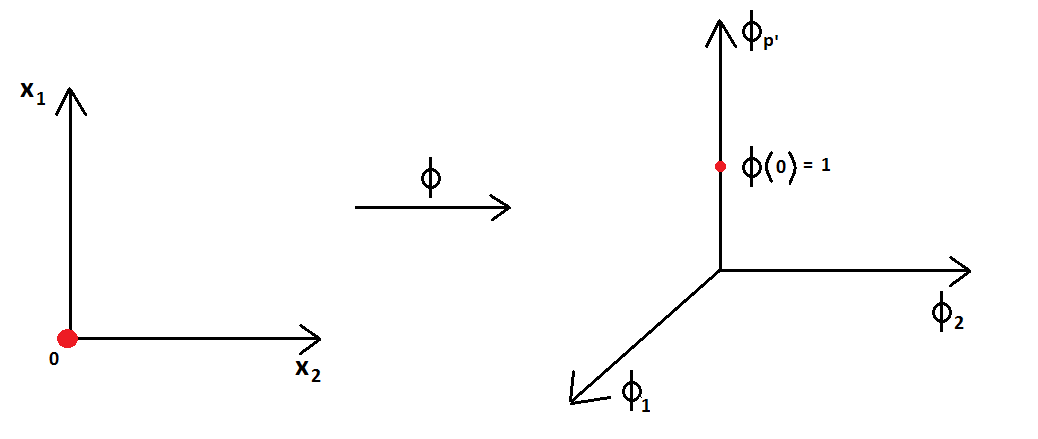
\includegraphics[width=0.9\linewidth]{images/Kernel_nonHomogene}
\caption{Illustration of samples in $\mathbb{R}^2$. The transformation $\phi$ for a polynomial kernel $K(\textbf{x}_i,\textbf{x}_j)=(\textbf{x}_i^T \textbf{x}_j + c)^d$ with $c=1$ and $d=2$ can be written explicitly: $\phi(\textbf{x}_i)= [x_{i1}^2, x_{i2}^2, \sqrt{2} x_{i1} x_{i2}, 1]^T$. The origin point $\textbf{x}_i=[0,0]^T$ is projected in the Hilbert space as $\phi(\textbf{x}_i=\textbf{0}) = [0, 0, 0, 1]^T$.}
\label{fig:Kernel_nonHomogene}
\end{figure}

However, to define proper metrics that respects the properties of metrics (Section \ref{sec:property_metric}), specific kernels must be used. Our work don't propose any solutions to this problem but open the field for new research on this topic. 



\section{Support Vector Machine ({\sc svm}) approximation}
\subsection{Motivations}
%\begin{itemize}
%	\item Faire remarquer que le problème LP ressemble à un problème SVM
%	\item Faire la démonstration de l'équivalence (ou mettre la démonstration en annexe).
%	\item Expliquer les différences entre la résolution LP/QP et la résolution SVM. (ajout de sur-contraintes dans le problème SVM)
%	\item Expliquer pourquoi on va préférer le cadre SVM. Expliquer mathématiquement et avec des interprétations géométriques. 
%	\item Cadre connu
%	\item Utilisation de librairie standard de Machine Learning
%	\item Extension directe à l'apprentissage de métrique non linéaire grâce au kernel trick
%\end{itemize}

Many parallels have been studied between Large Margin Nearest Neighbors ({\sc lmnn}) and {\sc svm} (Section \ref{sec:LMNN_SVM}). Similarly, the proposed {\sc mld} approach can be linked to {\sc svm}: both are convex optimization problem based on a regularized and a loss term. {\sc svm} is a well known framework: its has been well implemented in many libraries (\textit{e.g.}, {\sc liblinear} \cite{Fan2008} and {\sc libsvm} \cite{Hsu2008}), well studied for its generalization properties and extension to non-linear solutions. \\
\indent Motivated by these advantages, we propose to solve the {\sc mld} problem by solving a similar {\sc svm} problem. Then, we can naturally extend {\sc mld} approach to find non-linear solutions for the metric $D$ thanks to the 'kernel trick'. 
In the following, we show the similarities and the differences between {\sc lp}/{\sc qp} and {\sc svm} formulation.

For a time series $\textbf{x}_i$, we define the set of pairs $\textbf{X}_{pi}=\{(\textbf{x}_{ij},y_{ij}) \text{ s.t. } j\rightsquigarrow i \text{ or } y_{ij}=+1\}$. It corresponds for a time series $\textbf{x}_i$ to the set of pairs with target samples $\textbf{x}_j$ ($k$ nearest samples of same labels $j\rightsquigarrow i$) or samples $\textbf{x}_l$ that has a different label from $\textbf{x}_i$ ($y_l \neq y_i$) . Identity pairs $\textbf{x}_{ii}$ are not considered. We refer to $\textbf{X}_{p}=\bigcup\limits_{i} \textbf{X}_{pi}$ and consider the following standard soft-margin weighted {\sc svm} problem on $\textbf{X}_p$ \footnote{the {\sc svm} formulation below divides the loss part into two terms similarly to asymetric {\sc svm}}: 
\begin{equation}
\begin{aligned}
&\displaystyle \argmin_{\textbf{w},b,\xi} 
\left\lbrace \frac{1}{2}||\textbf{w}||_2^2
+ C \sum\limits_{i,j,y_{ij=-1}}p_i^-\xi_{ij}
+ C \sum\limits_{i,j, y_{ij=+1}}p_i^+\xi_{ij} \right\rbrace \\
& \text{s.t.  }  y_{ij}(\textbf{w}^T\textbf{x}_{ij}+b) \geq 1-\xi_{ij}
\end{aligned}
\label{eq:SVMSofMarginProblem}
\end{equation}
\noindent where $p_i^-$ and $p_i^+$ are the weight factors for target pairs and pairs of different class.

\noindent  We show in the following that solving the {\sc svm} problem in Eq.~\ref{eq:SVMSofMarginProblem} for $\textbf{w}$ and $b$ solves a similar {\sc mld} problem in Eq.~\ref{eq:MMLPrimalL2} for $D(\textbf{x}_i,\textbf{x}_j)=\frac{1}{2}(\textbf{w}^T\textbf{x}_{ij}+b)$. If we set $p_i^+$ being the half of the number of targets of $\textbf{x}_i$ and $p_i^-$, the half of the number of time series $L$ of a different class than $\textbf{x}_i$:
\begin{align}
p_i^+ &= \frac{k}{2} = \sum_{j \rightsquigarrow i} \frac{1}{2} \label{eq:pi_plus}\\
p_i^- &= \frac{L}{2} = \frac{1}{2}\sum_l \frac{1+y_{il}}{2} \label{eq:pi_moins}
\end{align}
% \noindent Note that in the case of $Q$ balanced classes of size $N$,  $p_i^- = N (Q-1)$. 

\subsection{Similarities and differences in the constraints}
% \noindent \textbf{Equivalence in the constraints} \\
\noindent First, we recall the {\sc svm} constraints in Eq.~\ref{eq:SVMSofMarginProblem}:
\begin{equation*}
y_{ij}(\textbf{w}^T\textbf{x}_{ij}+b) \geq 1-\xi_{ij} 
\end{equation*}
\noindent These constraints can be split into two sets of constraints:
%\begin{equation*}
%\begin{aligned}
%y_{ij}(\textbf{w}^T\textbf{x}_{ij}+b) & \geq 1-\xi_{ij} \text{ \quad (same class)} \\
%y_{il}(\textbf{w}^T\textbf{x}_{il}+b) & \geq 1-\xi_{il} \text{ \quad  (different classes)}
%\end{aligned}
%\end{equation*}
%\noindent which is equivalent to:
\begin{equation*}
\begin{aligned}
-(\textbf{w}^T\textbf{x}_{ij}+b) & \geq 1-\xi_{ij} \text{ \quad (same class: $y_{ij}=-1$)} \\
(\textbf{w}^T\textbf{x}_{il}+b) & \geq 1-\xi_{il} \text{ \quad  (different classes: $y_{ij}=+1$)}
\end{aligned}
\end{equation*}
\noindent By defining $D(\textbf{x}_{ij})=\frac{1}{2}(\textbf{w}^T\textbf{x}_{ij}+b)$, this leads to:
\begin{equation*}
\begin{aligned}
-D(\textbf{x}_{ij}) & \geq \frac{1}{2}-\frac{\xi_{ij}}{2} \\
D(\textbf{x}_{il}) & \geq \frac{1}{2}-\frac{\xi_{il}}{2}
\end{aligned}
\end{equation*}  
\noindent By summing each constraint two by two, this set of constraints implies the following set of constraints: \\
\resizebox{1\linewidth}{!}{
	\begin{minipage}{\linewidth}
		\begin{eqnarray}
		\begin{cases}
		\bullet \forall i,j,k,l \text{ such that } y_{ij}=-1, \text{ and } y_{kl}=+1, i \neq j \text{ and } i \neq k: \\
		D(\textbf{x}_k,\textbf{x}_l)-D(\textbf{x}_i,\textbf{x}_j) \geq 1-\frac{\xi_{kl}+\xi_{ij}}{2}  \\
		\bullet \forall i,j,l \text{ such that } y_{ij}=-1, \text{ and } y_{il}=+1, i \neq j: \\
		D(\textbf{x}_i,\textbf{x}_l)-D(\textbf{x}_i,\textbf{x}_j) \geq 1-\frac{\xi_{il}+\xi_{ij}}{2}
		\end{cases}
		\label{eq:Rewriten_Constraints}
		\end{eqnarray}
	\end{minipage}
} \\

\noindent By defining $\xi_{ijl}=\frac{\xi_{ij}+\xi_{il}}{2}$, the second constraint in Eq.~\ref{eq:Rewriten_Constraints} from the {\sc mdl} formulation is the same as the constraints in the {\sc svm} formulation in Eq.~\ref{eq:MMLPrimalL2_constraints1}. 

\indent However, an additional set of constraints is present in the {\sc svm} formulation (first set of constraints in Eq.~\ref{eq:Rewriten_Constraints}) and not in the proposed {\sc mld}. Geometrically, this can be interpreted as superposing the neighborhoods of all samples $\textbf{x}_i$, making the union of all of their target sets $\textbf{X}_{pi}$, and then pushing away all imposters $\textbf{x}_{il}$ from this resulting target set. This is therefore creating "artificial imposters" $\textbf{x}_{kl}$ that don't violate the local target space of sample $\textbf{x}_k$, but are still considered as imposters because they invade the target of sample $\textbf{x}_i$ (because of the neighborhoods superposition) (Figure \ref{fig:Neighborhood_scaling_problem}). This is more constraining in the {\sc svm} resolution for the resulting metric $D$ especially if the neighborhoods have different spread. 
% To overcome this issue, we propose to scale all target spheres to 1 in the preprocessing set, such that the risk of over-constraining the problem is very much mitigated.

\begin{figure}[h!]
	\centering
	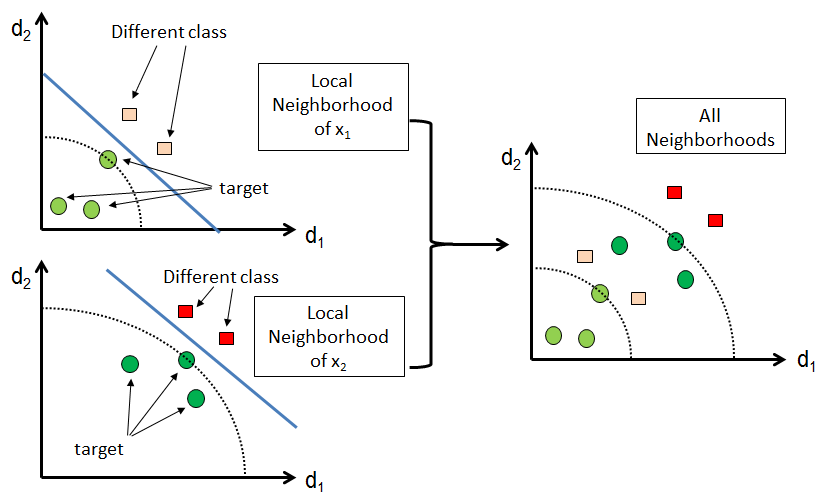
\includegraphics[width=0.8\linewidth]{images/Neighborhood_scaling_problem}
	\caption{Geometric representation of the neighborhood of $k=3$ for two time series $\textbf{x}_1$ and $\textbf{x}_2$ (left). For each neighborhood, time series of different class are represented by a square and the margin by a blue line. Taking each neighborhood separately, the problem is linearly separable ({\sc lp}/{\sc qp} formulation). By combining the two neighborhoods ({\sc svm} formulation), the problem is no more linearly separable and in this example, the time series of different class of $\textbf{x}_1$ (orange square) are "artificial imposters" of $\textbf{x}_2$. }
	\label{fig:Neighborhood_scaling_problem}
\end{figure}


\subsection{Similarities and differences in the objective function}
\label{sec:relationship}

% \noindent \textbf{Equivalence in the objective function} \\
\noindent Mathematically, from Eq. \ref{eq:pi_plus}, we write:
%\begin{equation}
\begin{align}
\sum\limits_{i,l,y_{il=+1}}p_i^+\xi_{il} 
& = 
\sum_{il}p_i^+   \frac{1+y_{il}}{2}  \xi_{il} \nonumber\\
& = 
\sum_{il} \left( \sum_{j \rightsquigarrow i} \frac{1}{2}\right)  \frac{1+y_{il}}{2}  \xi_{il} \nonumber\\
& =
\frac{1}{2}\sum_{i,j \rightsquigarrow i, l} \frac{1+y_{il}}{2}\xi_{il} \label{eq:pi_plus2}
\end{align}
%\end{equation}

\noindent And from Eq. \ref{eq:pi_moins}, we write:
\begin{align}
\sum\limits_{i,j, y_{ij=-1}}p_i^-\xi_{ij} 
& = 
\sum_{i,j \rightsquigarrow i}p_i^-\xi_{ij} \nonumber \\
& =
\sum_{i,j \rightsquigarrow i} \left( \frac{1}{2}\sum_l \frac{1+y_{il}}{2} \right) \xi_{ij} \nonumber \\
& =
\frac{1}{2}\sum_{i,j \rightsquigarrow i, l} \frac{1+y_{il}}{2}\xi_{ij} \label{eq:pi_moins2}
\end{align}

\noindent By replacing Eqs. \ref{eq:pi_plus2} and \ref{eq:pi_moins2} back into Eq. \ref{eq:SVMSofMarginProblem}, the objective function becomes:
%\begin{equation}
\begin{align}
&\displaystyle \min_{\textbf{w},\xi} 
\frac{1}{2}\textbf{w}^T \textbf{w}
 + C\sum_{i,j \rightsquigarrow i ,l}\frac{1+y_{il}}{2}\frac{\xi_{ij}+\xi_{il}}{2} \nonumber \\
&\displaystyle \min_{\textbf{w},\xi} 
\underbrace{ 
	\vphantom{ \sum\limits_{i,j \rightsquigarrow i,l} }
	\frac{1}{2}\textbf{w}^T \textbf{w}
}_{Regularization}
 + C \underbrace{
	\sum_{i,j \rightsquigarrow i ,l}
	\frac{1+y_{il}}{2} \xi_{ijl} 
}_{Loss}
\label{eq:svm2}
\end{align}	
%\end{equation} 
%\noindent The loss-function part of the {\sc svm} problem is similar to the one in Eq.~\ref{eq:MMLPrimalL2}. We can therefore use such {\sc svm}s with kernels to find non-linear forms for the metric $D$:
%
%\begin{align}
%D(\textbf{x}_{i'},\textbf{x}_{j'}) &= \frac{1}{2} 
%\left( \sum\limits_{ij} \alpha_{ij} 	
%y_{ij} 
%K
%\left( 
%\textbf{x}_{ij}
%,	
%\textbf{x}_{i'j'}
%\right) 
%+ b \right) 
%\label{Eq:nonlinearDSVM}		
%\end{align}

%In this section, we investigate the similarities and the differences between the {\sc lp}/{\sc qp} and {\sc svm} formulations. \\
\indent Even if the loss part (push cost) is the same for both objective functions, the regularization part (pull cost) is different. In the {\sc svm} formulation (Eq. \ref{eq:svm2}), the regularization part tends to minimize the norm of $\textbf{w}$ whereas in {\sc mld} (Eq.~\ref{eq:MMLPrimalL2}), it tends to minimize the norm of $\textbf{w}$ after a linear transformation through $\textbf{X}_{tar}$. This transformation can be interpreted as a Mahalanobis norm in the dissimilarity space with $\textbf{M}=\textbf{X}_{tar}\textbf{X}_{tar}^T$. Nevertheless, both have the same objective: improve the conditioning of the problem by enforcing solutions with small norms. In practice, even with these differences, the {\sc svm} provides suitable solutions for our time series metric learning problem. \\
%($\textbf{X}_{tar}.\textbf{X}_{tar}^T$ can be seen as a specific choice of Tikhonov matrix). 

\subsection{Geometric interpretation}
\todo[inline]{Michèle pense que l'état, cette section est dure à comprendre. D'après Michèle, il faut 1) soit prendre + de place pour expliquer la signification géométrique 2) ou soit ne pas mettre cette partie car étant compliquée, cela pourrait nuire au lecteur. Qu'en penses tu Ahlame?}
In this section, we give a geometric understanding of the differences between {\sc lp}/{\sc qp} resolution (left) and {\sc svm}-based resolution (right). Fig. \ref{fig:Linear} shows the Linear Programming ({\sc lp}) and {\sc svm} resolutions of a $k$-NN problem with $k=2$ neighborhoods. \\

For {\sc lp}, the problem is solved for each neighborhood (blue and red) independently as shown in Fig. \ref{fig:LP_separate}. We recall that {\sc lp}/{\sc qp} resolutions, support vectors are triplets of time series made of a target pair $\textbf{x}_{ij}$ and a pair of different classes $\textbf{x}_{il}$ (black arrows). Support vectors represent triplet which resulting distance $D(\textbf{x}_{ij}, \textbf{x}_{il})$ are the lowest. The optimization problem tends to maximize the margin between these triplets. The global solution (Fig. \ref{fig:Linear} (left)) is a compromise of all of the considered margins. In this case, the global margin is equal to one of the local margin. Note that the global {\sc lp} solution is not always the same as the best local solution. For {\sc svm}-based resolution (Fig. \ref{fig:Linear} (right)), the problem involves all pairs and the margin is optimized so that pairs $\textbf{x}_{ij}$ and $\textbf{x}_{il}$ are globally separated.



\begin{figure}[h!]
	\centering
	\begin{minipage}[b]{1\linewidth}
		\centerline{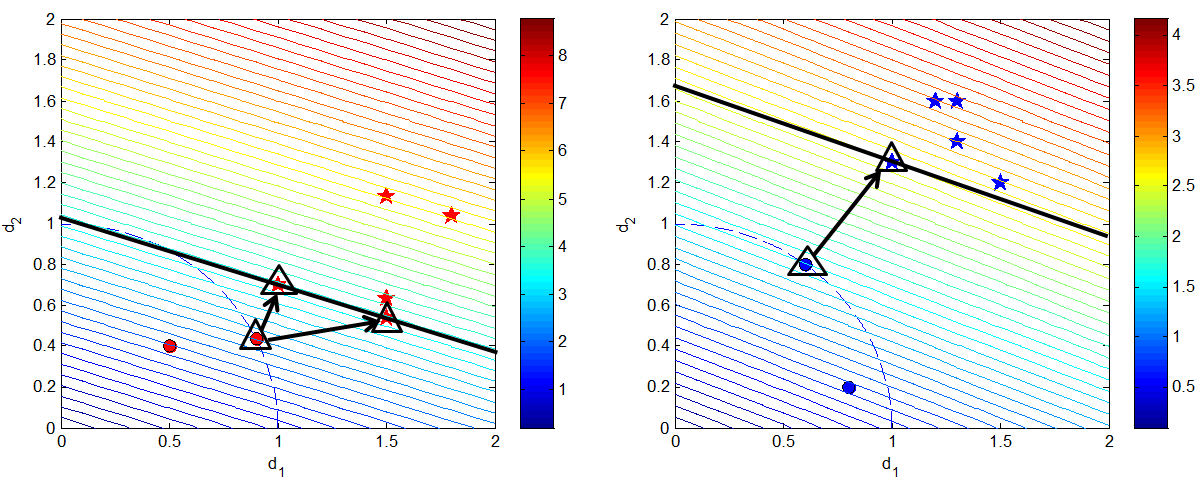
\includegraphics[width=1\linewidth]{images/InterpretationLP}}
	\end{minipage}
	\caption{Solutions found by solving the {\sc lp} problem for $k=2$ neighborhood. Positive pairs (different classes) are indicated in stars and negative pairs (target pairs) are indicated in circle. Red and blue lines shows the margin when solving the problem for each neighborhood (red and blue points) separately. Support vector are indicated in black triangles: in the red neighborhood (left), 2 support vectors are retained and in the blue neighborhood (right), only one support vector is necessary.}
	\label{fig:LP_separate}
\end{figure}

\begin{figure}[h!]
	\centering
	\begin{minipage}[b]{1\linewidth}
		\centerline{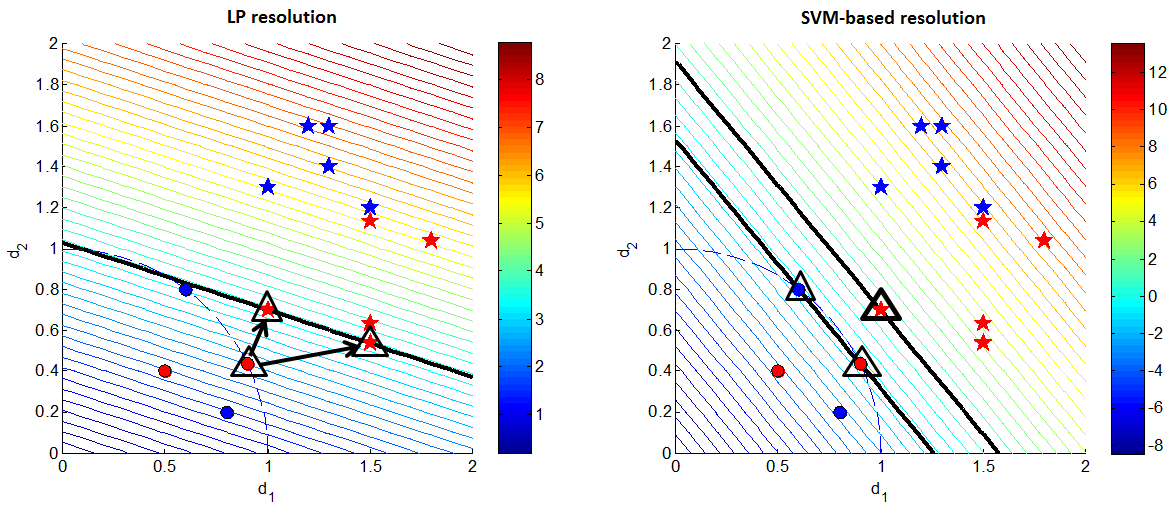
\includegraphics[width=1\linewidth]{images/InterpretationLP_SVM}}
	\end{minipage}
	\caption{Solutions found by solving the {\sc lp} problem (left) and the {\sc svm} problem (right). The global margin is indicated in black and the metric is represented in color levels. Support vectors made of triplets are indicated in black triangles. For the {\sc svm}, the black lines indicates the {\sc svm} canonical hyperplane where the support vector lies (black triangles).}
	\label{fig:Linear}
\end{figure}

\newpage
\section{Conclusion of the chapter}
To learn a combined metric $D$ from several unimodal metrics $d_h$ that optimizes the $k$-NN performances, we first proposed a new space representation, the dissimilarity space where each pair of time series is projected as a vector described the unimodal metrics. Then, we propose three formalizations of our metric learning problem: Linear Programming, Quadratic Programming, {\sc svm}-based approximation. Table \ref{tab:resume_methode} sums up the main pros and cons of each formulation.

\begin{table}[h!]
	\small
	\centering
	\renewcommand{\arraystretch}{0.85}
	\resizebox{0.6\textwidth}{!}{
		\setlength{\tabcolsep}{1pt}
		\begin{tabular}{lccc}
			\hline
									& LP	& QP 	& SVM-based\\
			\hline
			Linear 					& Yes	& Yes 	& Yes 		\\
			Non-linear extension 	& No	& Yes 	& Yes 		\\
			Exact/Approximation resolution	& Exact	& Exact	& Approximation \\
			Sparcity 				& Yes	& No    & Yes/No 	\\
			\hline
		\end{tabular}}
		\caption{The different formalizations for Metric Learning in Dissimilarity space}
		\label{tab:resume_methode}
\end{table}
  
In the following, we consider the {\sc svm}-based approximation because {\sc svm} framework is well known and well implemented. In the next chapter, we give the details of the steps of our proposed algorithm: Multi-modal and Multi-scale Time series Metric Learning ({\sc m}$^2${\sc tml}).

